% This is samplepaper.tex, a sample chapter demonstrating the
% LLNCS macro package for Springer Computer Science proceedings;
% Version 2.20 of 2017/10/04
%
\documentclass[runningheads]{llncs}
%
%\usepackage{graphicx}
% Used for displaying a sample figure. If possible, figure files should
% be included in EPS format.
%
% If you use the hyperref package, please uncomment the following line
% to display URLs in blue roman font according to Springer's eBook style:
% \renewcommand\UrlFont{\color{blue}\rmfamily}

% 1. Preamble and packages
\usepackage{lipsum}
\usepackage{amsfonts}
\usepackage{graphicx}
%\usepackage{epstopdf}
%\usepackage{algorithmic}

% Tools for mathematical typesetting
\usepackage{algpseudocode} 
% Typesetting algorithms
\usepackage{algorithm}

\usepackage{amsmath}

% ++++ Vectors
\def \vepsilon{ \boldsymbol{\varepsilon} }
\def \vu{ \boldsymbol{u} }
\def \vU{ \boldsymbol{U} }
\def \vzeta{ \boldsymbol{\zeta} }
\def \vx{ \mathbf{x} }
\def \vp{ \boldsymbol{p} }
\def \vs{ \boldsymbol{s} }
\def \vn{ \boldsymbol{n}}
\def \vf{ \boldsymbol{f} }
\def \vxi{\boldsymbol{\xi}}
\def \vom{\boldsymbol{\omega}}

\def \Hx { \hat{1} }
\def \Hy { \hat{2} }
\def \Ht{ \hat{t} }
\def \Hu{ \hat{u} }
\def \Hv{ \hat{v} }
\def \Hw{ \hat{w} }
\def \vc { \boldsymbol{c} }

\def \vn{ \boldsymbol{n} }
\def \vW{ \boldsymbol{W} }
\def \vv{ \mathbf{v} }
\def \vb{ \mathbf{b} }
\def \ve{ \mathbf{e} }
\def \vz{ \mathbf{z} }

\def \vsig{ \boldsymbol{\sigma}}
\def \tnsrsig{ \underset{\thickapprox}{\boldsymbol{\sigma} }}
\def \tnsreps{\underset{\thickapprox}{\boldsymbol{\varepsilon} }}

%  +++++ Tensors
\def \tnsrsig{ \underset{\thickapprox}{\boldsymbol{\sigma} }}
\def \tnsreps{\underset{\thickapprox}{\boldsymbol{\varepsilon} }}
%  +++++ Operators
\def\calB{{\mathcal B}}
\def\calF{{\mathcal F}}
\def\calU{{\mathcal U} }
\def\calUvu{ \mathcal U(\vu) }
\def\calR{\mathcal R }
\def\calS{{ \mathcal S}}
\def\calE{{ \mathcal E}}
\def\calD{{ \mathcal D}}
\def\calP{{ \mathcal P}}
\def\calI{{ \mathcal I}}
\def\calG{{ \mathcal G}}
\def\calL{{ \mathcal L}}

\def \vX{ \mathbf{x} }
\def \vY{ \mathbf{y} }
\def \vg{ \mathbf{g} }
\def \vq {\mathbf{q} }

%**************************************
\newcommand{\alp}[3]{{\left . \alpha_{#1} \right |^{#2}_{#3}\ }}
\newcommand{\bet}[3]{{\left .  \beta_{#1} \right |^{#2}_{#3}\ }}
\newcommand{\Balp}[3]{{\left . \BM {\alpha}_{#1} \right |^{#2}_{#3}\ }}
\newcommand{\Bbet}[3]{{\left . \BM {\beta}_{#1} \right |^{#2}_{#3}\ }}
\newcommand{\Bzet}[2]{{\BM {\zeta}^{#1}_{#2}}}
\newcommand{\B}[1]{{\underline{#1}}}
\newcommand{\Bf}[1]{\boldsymbol{#1}}
\newcommand{\Bc}[1]{\mathcal{#1}}
\newcommand{\Bd}[1]{\mathbb{#1}}
\newcommand{\Bs}[1]{\mathsf{#1}}
\newcommand{\dif}{\mathrm{d}}
\newcommand{\pdif}[2]{\frac{\partial {#1}}{\partial {#2}}}
\newcommand{\pfrac}[2]{\frac{\partial {#1}}{\partial {#2}}}
\newcommand{\scite}[1]{\textsuperscript{\cite{#1}}}
\newcommand{\ul}{\underline}
\newcommand{\II}{\ensuremath{I \hspace{-0.2em} I}}
\newcommand{\III}{\ensuremath{I \hspace{-0.2em} I \hspace{-0.2em} I}}
\newcommand{\CI}{\mathbf{C} \hspace{-0.6em} \mbox{\small I} }
\newcommand{\ci}{\mathbf{c} \hspace{-0.6em} \mbox{\small I} }
\newcommand{\ljump}{\left [  \hspace{-0.21em} \left | }
\newcommand{\rjump}{\right | \hspace{-0.21em} \right ]}
\newcommand{\odif}[2]{\frac{\mathrm{d}  {#1}}{\mathrm{d} {#2}}}
\newcommand{\into}{ \int_{\Omega}}
\newcommand{\difo}{ \;\mathrm{d}\Omega}
\newcommand{\difg}{ \;\mathrm{d}\Gamma}
\newcommand{\BM}[1]{\mbox{\boldmath $#1$}}
\newcommand{\BMB}[1]{\mbox{$\mathbb #1$}}
%\newcommand{\BM}[1]{\mbox{$\mathbf  #1$}}
\newcommand{\bdiff}{\BM{\cal D}}
\newcommand{\diff}{{\cal D}}
\newcommand{\<}{\langle}
\renewcommand{\>}{\rangle}
\newcommand{\Nel}{N_{el}}
\newcommand{\smfrac}[2]{\mbox{$\frac{#1}{#2}$}}


\newcommand{\lon}{\lambda}
\newcommand{\lat}{\theta}
\newcommand{\lond}{\lambda}
\newcommand{\latd}{\theta}
\newcommand{\lons}{\lambda^{\rm e}}
\newcommand{\lats}{\theta^{\rm e}}
\newcommand{\lf}{\left}
\newcommand{\rt}{\right}
\newcommand{\lp}{\lf (}
\newcommand{\rp}{\rt )}
\newcommand{\ep}{\varepsilon}
\newcommand{\tngt}{\boldsymbol{\tau}}
\newcommand{\utngt}{\hat{\boldsymbol{\tau}}}
\newcommand{\unrml}{\hat{\boldsymbol{\eta}}}
\newcommand{\frc}{\mathbf{F}}
\newcommand{\matlab}{\textsc{Matlab\;}}
\newcommand{\inner}[2]{\langle #1,#2 \rangle}

\def \div{D \cdot}
\def \Xd{ X^{\rm d} }
\def \Xs{ X^{\rm s} }
\def \Yd{ Y^{\rm d} }
\def \Ys{ Y^{\rm s} }
\def \vXd{ \boldsymbol{X}^{\rm d} }
\def \vXs{ \boldsymbol{X}^{\rm s} }
\def \ucd{ \vec{\alpha}^X_{\rm d} }
\def \ucdb{ \vec{\alpha}^Y_{\rm d} }
\def \uXd{ \vec{X}_{\rm d}(t) }
\def \uvXd{ \vec{\vX}_{\rm d} }
\def \uvXs{ \vec{\vX}_{\rm s} }
\def \uYd{ \vec{Y}_{\rm d}(t) }
\def \uXs{ \vec{X}_{\rm s}(t) }

% ++++ Vectors.
\def \vepsilon{ \boldsymbol{\varepsilon} }
\def \vu{ \boldsymbol{u} }
\def \vU{ \boldsymbol{U} }
\def \vzeta{ \boldsymbol{\zeta} }
\def \vx{ \boldsymbol{x} }
\def \va{ \boldsymbol{a} }
\def \vy{ \boldsymbol{y} }
\def \vn{ \boldsymbol{n}}
\def \vt{ \boldsymbol{t}}
\def \vf{ \boldsymbol{f} }
%\def \vX{ \boldsymbol{X} }
\def \vc{ \mathbf{c} }
\def \vd{ \mathbf{d} }
\def \vP{ \boldsymbol{P} }
\def \vB{ \boldsymbol{B} }
\def \vp{ \boldsymbol{p} }
\def \vF{ \boldsymbol{F} }

\def \vs{ \mathbf{s}}

\def \Hx { \hat{1} }
\def \Hy { \hat{2} }
\def \Ht{ \hat{t} }
\def \Hu{ \hat{u} }
\def \Hv{ \hat{v} }
\def \Hw{ \hat{w} }
\def \Htau{ \hat{\tau} }
\def \vhtau{ \boldsymbol{\Htau} }
\def \vc { \boldsymbol{c} }
\def \vr { \mathbf{r} }
\def \ve{ \boldsymbol{e} }
\def \vW{ \boldsymbol{W} }
\def \vv{ \mathbf{v} }

\def \vsig{ \boldsymbol{\sigma}}
\def \tnsrsig{ \underset{\thickapprox}{\boldsymbol{\sigma} }}
\def \tnsreps{\underset{\thickapprox}{\boldsymbol{\varepsilon} }}
\newcommand{\calp}{\mathbf{p}}
\newcommand{\Erbf}{E_{\rm rbf}}
\def\bicgstab{{BICGSTAB}} 


% ++++ Vectors.
\def \vepsilon{ \boldsymbol{\varepsilon} }
\def \vu{ \boldsymbol{u} }
\def \vU{ \boldsymbol{U} }
\def \vzeta{ \boldsymbol{\zeta} }
\def \vx{ \boldsymbol{x} }
\def \vn{ \boldsymbol{n}}
\def \vf{ \boldsymbol{f} }
\def \vX{ \boldsymbol{X} }
\def \vZ{ \boldsymbol{Z} }
\def \vXd{ \boldsymbol{X}^{\rm d} }
\def \vXs{ \boldsymbol{X}^{\rm s} }
\def \vY{ \boldsymbol{Y} }
\def \vc{ \boldsymbol{c} }
\def \vP{ \boldsymbol{P} }
\def \vF{ \boldsymbol{F} }

% scalars
\def \Xd{ X^{\rm d} }
\def \Xs{ X^{\rm s} }
\def \Yd{ Y^{\rm d} }
\def \Ys{ Y^{\rm s} }
\def \Zd{ Z^{\rm d} }
\def \Zs{ Z^{\rm s} }

\def \Hx { \hat{1} }
\def \Hy { \hat{2} }
\def \Ht{ \hat{t} }
\def \Hu{ \hat{u} }
\def \Hv{ \hat{v} }
\def \Hw{ \hat{w} }
\def \Htau{ \hat{\tau} }

% Grady's commands
\def \ucd{ \vec{c}^X_{\rm d} }
\def \uXd{ \vec{X}_{\rm d}(t) }
\def \uvXd{ \vec{\vX}_{\rm d} }
\def \uvXs{ \vec{\vX}_{\rm s} }
\def \uYd{ \vec{Y}_{\rm d}(t) }
\def \uXs{ \vec{X}_{\rm s}(t) }
\def \uTd{ \vec{T}_{\rm d} }
\def \uvZd{ \vec{\vZ}_{\rm d} }
\def \uvFs{ \vec{\vF}_{\rm s} }
\def \uvFTs{ \vec{\vF}_{\rm s}^{\rm T} }
\def \uvFBs{ \vec{\vF}_{\rm s}^{\rm B} }
\def \uvFCs{ \vec{\vF}_{\rm s}^{\rm C} }
\def \tngtd{ \tngt_{\rm d} }
\def \utngtd{ \vec{\tngt}_{\rm d} }
\def \uutngtd{ \vec{\hat{\tngt}}_{\rm d} }
\def \utngtslon{ \vec{\tngt}_{\rm s}^{\lon} }
\def \utngtslat{ \vec{\tngt}_{\rm s}^{\lat} }
\def \uunrmls{ \vec{\unrml}_{\rm s} }
\def \Es{ \mathcal{E}_{\rm s} }
\def \ub{ \vec{b}_{\lon} }
\def \ubd{ \ub^{n} }
\def \ubs{ \vec{b}_{\lon,\lat} }
\def \ubsd{ \ubs^{m,n} }
\newcommand{\Dlond}[1]{\mathcal{D}_{\lond}^{#1}}
\newcommand{\Dlons}[1]{\mathcal{D}_{\lons}^{#1}}
\newcommand{\Dlonlatd}[2]{\mathcal{D}_{\lond,\latd}^{#1,#2}}
\newcommand{\Dlonlats}[2]{\mathcal{D}_{\lons,\lats}^{#1,#2}}
\newcommand{\ds}{\displaystyle}
\newcommand{\Sph}{\mathbb{S}^2}

\def \vhtau{ \boldsymbol{\Htau} }
\def \vc { \boldsymbol{c} }
\def \vn{ \boldsymbol{n} }
\def \vW{ \boldsymbol{W} }
\def \vv{ \mathbf{v} }
\def \vsig{ \boldsymbol{\sigma}}
\def \tnsrsig{ \underset{\thickapprox}{\boldsymbol{\sigma} }}
\def \tnsreps{\underset{\thickapprox}{\boldsymbol{\varepsilon} }}

%  +++++ Tensors
\def \tnsrsig{ \underset{\thickapprox}{\boldsymbol{\sigma} }}
\def \tnsreps{\underset{\thickapprox}{\boldsymbol{\varepsilon} }}

%  +++++ Operators
\def\calA{{\mathcal A}}
\def\calB{{\mathcal B}}
\def\calF{{\mathcal F}}
\def\calU{{\mathcal U} }
\def\calUvu{ \mathcal U(\vu) }
\def\calR{\mathcal R }
\def\calS{{ \mathcal S}}
\def\calE{{ \mathcal E}}
\def\calD{{ \mathcal D}}

\newcommand{\Nd}{N_{\rm d}}
\newcommand{\Ns}{N_{\rm s}}
\newcommand{\frcT}{\frc^{\rm T}}
\newcommand{\frcB}{\frc^{\rm B}}
\newcommand{\frcC}{\frc^{\rm C}}
\newcommand{\kt}{k_{\rm t}}
\newcommand{\kb}{k_{\rm b}}
\newcommand{\KC}{K_{\rm C}}
\newcommand{\ellC}{l_{0,\rm C}}

%\let\oldenumerate\enumerate
%\renewcommand{\enumerate}{
%  \oldenumerate
%  \setlength{\itemsep}{1pt}
%  \setlength{\parskip}{0pt}
%  \setlength{\parsep}{0pt}
%}

%\let\olditemize\itemize
%\renewcommand{\itemize}{
%  \olditemize
%  \setlength{\itemsep}{1pt}
%  \setlength{\parskip}{0pt}
%  \setlength{\parsep}{0pt}
%}

% Notation for the augmented RBF system (which is a saddle point)
\newcommand{\Asp}{\widetilde{A}}
\newcommand{\csp}{\widetilde{\vc}}
\newcommand{\fsp}{\widetilde{\vf}}

\newcommand{\comment}[1]{{\color{red}{[#1]}}}
%\ifpdf%
%  \DeclareGraphicsExtensions{.eps,.pdf,.png,.jpg}
%\else
%  \DeclareGraphicsExtensions{.eps}
%\fi
\usepackage{amsopn}
\usepackage{amssymb}
\DeclareMathOperator{\diag}{diag}
\usepackage{booktabs}
\usepackage{float}

\newcommand{\bs}[1]{\ensuremath{\boldsymbol #1}}
\newcommand{\mynote}[3]{
	\textcolor{#2}{\fbox{\bfseries\sffamily\scriptsize#1}}
		{\small$\blacktriangleright$\textsf{\emph{#3}}$\blacktriangleleft$}
}

\newcommand{\mr}[1]{\mynote{Majid}{blue}{#1}}
\newcommand{\hs}[1]{\mynote{Hari}{olive}{#1}}


\begin{document}
%
\title{Lazy-update Multigrid Preconditioners}
%
\titlerunning{Abbreviated paper title}
% If the paper title is too long for the running head, you can set
% an abbreviated paper title here
%
\author{Majid Rasouli\inst{1,2} %\orcidID{0000-1111-2222-3333}
\and Vidhi Zala\inst{1,3} %\orcidID{1111-2222-3333-4444}
\and Robert M. Kirby\inst{1,4} %\orcidID{2222--3333-4444-5555}
\and Hari Sundar\inst{1,5} %\orcidID{2222--3333-4444-5555}
}
%
\authorrunning{M. Rasouli et al.}
% First names are abbreviated in the running head.
% If there are more than two authors, 'et al.' is used.
%
\institute{School of Computing, University of Utah, SLC, UT, USA \\
\and
\email{rasouli@cs.utah.edu}\\
%\url{https://www.cs.utah.edu/~rasouli/}
\and
%ABC Institute, Rupert-Karls-University Heidelberg, Heidelberg, Germany\\
\email{vidhi@sci.utah.edu}
\and
\email{kirby@sci.utah.edu}
\and
\email{hari@cs.utah.edu}
}
%
\maketitle              % typeset the header of the contribution
%
\begin{abstract}
Multigrid is one of the most effective methods for solving elliptic PDE’s. 
It is algorithmically optimal and is robust when combined with Krylov methods. 
Algebraic multigrid is especially attractive due to its blackbox nature. This 
however comes at the cost of increased setup costs that can be significant in 
case of systems where the system matrix changes frequently making it difficult 
to amortize the setup cost. In this work, we investigate several strategies for 
performing lazy updates to the multigrid hierarchy corresponding to changes in 
the system matrix. These include delayed updates, value updates without changing 
structure, process local changes, and full updates. We demonstrate that in many 
cases, the overhead of building the AMG hierarchy can be mitigated for rapidly 
changing system matrices.

\keywords{Algebraic Multigrid \and Iterative Solver \and Sparse \and Preconditioned Conjugate Gradient \and Preconditioner}
\end{abstract}
%

\section{Introduction}
\label{sec:intro}

The solution of elliptic partial differential equation (PDE) operators forms the 
foundation of the mathematical models of several engineering applications.
In solid mechanics, the stiffness matrix derived from linear elasticity represents an elliptic
operator that, when discretized with the finite element method (FEM) yields a symmetric positive
definite system. In fluid mechanics, the viscous terms and the pressure components of
the incompressible Navier-Stokes equations, when discretized, often lead to symmetric
positive definite systems. 
For the solution of such large-scale systems that need to be solved in parallel, iterative solvers 
with $\mathcal{O}(n)$ complexity and mesh-independent convergence are preferred. 
%
The most popular methods in this regard have been the multigrid methods--both geometric and algebraic. 
The geometric multigrid (GMG) methods when applied
to matrices generated from regular (often evenly-spaced) discretizations of elliptic operators \cite{MadayMunoz88,BrambleZhang00,Brenner02,GholamiMalhotraSundar2016}.
The mathematical predictability of the benefits of the GMG approach combined with the ability to
exploit the regularity of the data structures (in terms of indexing, coarsening, etc.) has made
GMG, especially in conjunction with preconditioned conjugate gradient (PCG) \cite{Braess86,TatebeOyanagi94}, the solver of choice when solving engineering applications that require large-scale
parallel solution approaches.  The story is more mixed when one moves to unstructured discretizations
and corresponding to algebraic multigrid (AMG), the communities alternative to GMG for such problems.  

While AMG is very attractive due to its black-box nature \cite{Dendy82,Vanek:1995,VanekBrezinaMandelEtAl01}, it does not scale as well as GMG \cite{Sundar12}. This is primarily due to
the loss of sparsity at coarser levels arising from the Galerkin approximation \cite{treister2015non}, leading to poor scalability, especially at the coarser levels.
Additionally, while both geometric and algebraic variants require an initial {\bf setup} phase, the cost of the setup is significantly higher for AMG, making it less attractive unless multiple solves are performed for the same operator. This is clearly unattractive for dynamic systems where the operator is changing rapidly, such as systems with $h$ or $p$ enrichment. In such cases, while the cost of an AMG solve might be lower than say that of CG, the overall cost i.e., setup + solve might be more than using asymptotically inferior solvers. In most cases, the scalbility of 
setup phase is also poor and typically worse than that of the solve phase. This is limited the attractiveness of AMG for large systems. In this work, we develop an efficient sparse matrix multiplication (\mm) algorithm to improve the performance and scalability of AMG. As will be explained in the following section, a sparse \mm\ is the dominant part of the AMG setup. While several of our optimizations apply to sparse \mm\ in general, and can be more broadly applied, our strategies for reducing inter-process communication make use of the special structure of \mm\ encountered during AMG setup.

\subsection{Background}
\label{sec:bg}

We start with a brief description of our AMG framework. 
AMG has been a popular method for solving the large-scale and 
often sparse linear system one obtains from discretization of elliptic partial 
differential equations.  The linear system can be written as
\begin{equation}
 Ax = b
\end{equation}
\noindent in which, $A \in R^{n \times n}$, $x$ and $b \in R^{n}$.
AMG consists of a setup and a solve phase.
%Three different sets of matrices will be created during the setup phase,
%and they will be used in the solve phase to solve the linear system.
The first step of the setup phase is to aggregate the nodes of the equivalent 
graph ($G$) of the matrix $A$. Every row of the matrix $A$ is considered as a node
in the graph $G$ and there is an edge between nodes $i$ and $j$ if entry $(i,j)$ is nonzero in $A$.
%This next sentence does not make sense - "By doing the aggregation on them??".  
After aggregation, %By doing the aggregation on them, 
some nodes will be chosen as \textit{roots} and the
rest of the nodes of the graph will be assigned to them.
Multiple aggregation methods for AMG have been introduced, such as
\cite{bell2012exposing}, \cite{notay2010aggregation},
\cite{Guillard98anaggregation}, %\cite{DBLP:journals/siamsc/SalaT08}, \cite{Vanek:1995}
\cite{DBLP:journals/siammax/Notay06}. %\cite{DBLP:journals/siamsc/Notay12}, \cite{BrezinaFMMMR05}, \cite{Brezina}
\hl{For this paper}, \textit{2-distance maximal independent set} from \cite{bell2012exposing}, with some modifications, is used. \mr{Check and correct.}

Given a linear system we have $n$ 
nodes in the graph $G$ and $m$ nodes are chosen as the \textit{roots}.
We compute prolongation $P$ and Restriction $R$ operators using the \textit{roots}. 
%A matrix, called the \textit{prolongation matrix} $P$, of size $n \times m$ is defined based on these nodes. If node $i$ is assigned to root $j$, then $P(i,j) = 1$, otherwise it is $0$. The restriction matrix $R \in R^{m \times n}$ is then made by transposing $P$.
The prolongation operator has two applications. It can interpolate a vector $v \in R^m$ to $v' \in R^n$, such that $m < n$.
The other application is creating a coarse version of the operator $A$ using the Galerkin approximation:

\begin{equation}
  \label{eq:rap}
 A_c = R \times A \times P
\end{equation}

\noindent such that $A_c \in R^{m \times m}$. This operation is called \textit{coarsening}.
The restriction operator is used similarly. The triple \mm\ in (\ref{eq:rap}) is the dominant cost of the AMG setup, especially when done in parallel. Improving the efficiency and scalability of this step in the main contribution of this work. 
%; in addition to being used in the coarsening, it takes a vector $w \in R^n$ to $R^m$.

Progressively coarser versions of the matrix are created during the setup phase corresponding to
a hierarchy (i.e. multi-level or ``multigrid") of data structures.
An AMG hierarchy of $L+1$ levels consists of three categories of operators:
coarse matrices ($As$), prolongation matrices ($Ps$) and restriction matrices ($Rs$).

%\begin{enumerate}
% \item \underline{Coarse Matrices}:       $As[0]$, $As[1]$, ..., $As[L]$, where $As[0]$ represents the finest matrix $A$
% \item \underline{Prolongation Matrices}: $Ps[0]$, $Ps[1]$, ..., $Ps[L-1]$
% \item \underline{Restriction Matrices}:  $Rs[0]$, $Rs[1]$, ..., $Rs[L-1]$
%\end{enumerate}

The coarse matrices for each level are created similar to $A_c$:
\begin{equation*}
 As[l+1] = Rs[l] \times As[l] \times Ps[l],\ l = 0, 1, ..., L
\end{equation*}
such that $As[0]$ is the finest matrix $A$. Again note that this is very expensive even at the coarser levels as the matrices get denser at the coarser levels. Our \mm\ maintains good performance and scalability across all levels of the multigrid hierarchy. 

The next phase of AMG is the solve phase. To solve $Ax = b$, we start with an initial guess for $x$.
% Two methods are utilized in the solve phase to find the approximate solution:
% \begin{enumerate}
%  \item Relaxation
%  \item Coarse-Grid Correction (CGC)
% \end{enumerate}

% Algorithm \ref{alg:amg} shows the AMG loop, which repeats until the solution is found within the 
% desired accuracy. The grid $g$ is the AMG hierarchy, consisting the three matrix categories mentioned previously.
% %of the coarse matrices ($As$), prolongation operators ($Ps$), and restriction operators ($Rs$).

% \begin{algorithm}[ht] 
%   \caption{AMG} \label{alg:amg} 
%   \begin{algorithmic}[1]
%     \Require $grid\ (g)$, $b$ and $initial\ guess\ (x_0)$
%     \Ensure  $solution\ (x)$
%     \While{not converged}
%       \State $x \leftarrow\ vcycle(g,\ x_0,\ b,\ 0$)
%     \EndWhile
%   \end{algorithmic}
% \end{algorithm}
The solution is computed in a recursive function \textit{vcycle} (Algorithm \ref{alg:vcycle}).
Regular smoothers are used in the relaxation part, such as Jacobi, Chebyshev, etc.
Then, the residual $r$ is computed. Next, $r$ is taken to the coarser level by using
the restriction operator ($R$).
The function recurses until it reaches the coarsest level ($L+1$). At that level,
the system will be solved directly. The solution of that system is actually the error,
which will be interpolated by $P$.
After that, the solution will be corrected by subtracting the interpolated error from it.
Finally, the solution will be smoothed again.

\begin{algorithm}[ht] 
  \caption{vcycle($g, x,\ b,\ l$)} \label{alg:vcycle} 
  \begin{algorithmic}[1]
    \Require $grid\ g$, $b$, $x$, and $level\ (l)$
    \Ensure  $solution\ (x)$
    \If{$l = L+1$}
      \State $x \leftarrow direct\ solver(g[L+1],\ x,\ b)$
    \Else
      \State $x \leftarrow Smoother(g, x,\ b,\ l)$
      \State $r \leftarrow As[l] \times x - b$
      \State $r_c \leftarrow Rs[l] \times r$
      \State $y_c \leftarrow$ $vcycle(g, x,\ r_c,\ l+1)$
      \State $y \leftarrow Ps[l] \times y_c$
      \State $x \leftarrow x - y$
      \State $x \leftarrow Smoother(g, x,\ b,\ l)$
    \EndIf
  \end{algorithmic}
\end{algorithm}

\textit{Smoothed Aggregation AMG (SA-AMG)}\cite{Vanek:1995} is a modified version of AMG,
in which the prolongation and restriction operators are smoothed %, for instance by the Jacobi method,
to improve the convergence of AMG.
For this paper, the improved version of SA-AMG in \cite{treister2015non} is used.

\begin{itemize}
  \item \st{General intro to AMG and elliptic operators, black box nature.}
  \item \st{General outline of AMG method, setup and solve.}
  \item \st{Why setup costs are important, what dominates}
  \item what others have done.
  \item This work and contributions.
  \item rest of the paper.
\end{itemize}

\section{Methods}
\label{sec:methods}

In this section, we present our matrix-matrix multiplication algorithm, the choice of the stop condition for the recursive function and how matrices are being divided to smaller blocks. We then explain how the communication is being done in the distributed fashion to help the recursive function scale better.

%We then explain further modifications to the triple matrix multiplication (\ref{eq:rap}) that are part of the AMG setup process.

\subsection{Matrix-Matrix Multiplication}
\label{sec:matmult}

%\subsubsection{Computation}
%\label{sec:comp}
We design a divide and conquer approach to perform the sparse \mm\ in a node-local fashion. The key idea is to perform simple tasks while recursing, having efficient memory access, and to perform the multiplication for small chunks where the resulting matrix can fit into an appropriate cache. For clarity of presentation, we assume that the data is available locally and discuss it as a serial implementation. Shared memory parallelism is added in a straightforward manner.
%We have implemented \mm~ in a recursive fashion.
%We split the matrices recursively in two ways: split by half based on the matrix size and based on number of nonzeros. First we explain the algorithms performing splitting based on the matrix sizes.

To perform the multiplication
\begin{equation}
    C = A \times B
\end{equation}
we keep splitting the matrices horizontally and vertically (Figure~\ref{fig:split2}) based on row size and column size of $A$, until we can fit the result of the multiplication in a dense matrix.

\begin{figure}[tbh]
 \centering
 
\includegraphics[width=8.5cm,height=2.7cm]{./figures/split2.pdf}
 \caption{A basic scheme that shows splitting the matrix first horizontally, then vertically.}
 \label{fig:split2}
 \Description{}
\end{figure}

The recursive function, \recmm, includes three cases:
\begin{enumerate}
 \item Case 1: Stop the recursion: perform the multiplication.
 \item Case 2: $A$ is horizontal. Split $A$ and $B$.
 \item Case 3: $A$ is vertical. Split $A$ and $B$.
\end{enumerate}

\subsubsection{Case 1}
\label{sec:case1}
First we discuss when we decide to stop the recursive function.  
Our goal is to fit the multiplication result of blocks of $A$ and $B$ in a dense buffer. We show the blocks of $A$ and $B$ as $A_{ij}$ and $B_{lk}$. We use two indices here because matrices gets divided both horizontally and vertically. The size of the dense buffer to store $A_{ij} \times B_{lk}$ is
\begin{equation}
    row\ size\ of\ A_{ij} \times column\ size\ of\ B_{lk}\label{eq:thres}
\end{equation}

Therefore, the obvious choice to decide when to stop the recursion is Equation~ \eqref{eq:thres}, but Figure~\ref{fig:thres} shows why that is not a good choice. If we use Equation~ \eqref{eq:thres} for this example, the splitting process for the top two blocks of the matrix stops at the same step, but the top left block should be divided to more blocks than the top right block.

\begin{figure}[tbh]
 \centering
 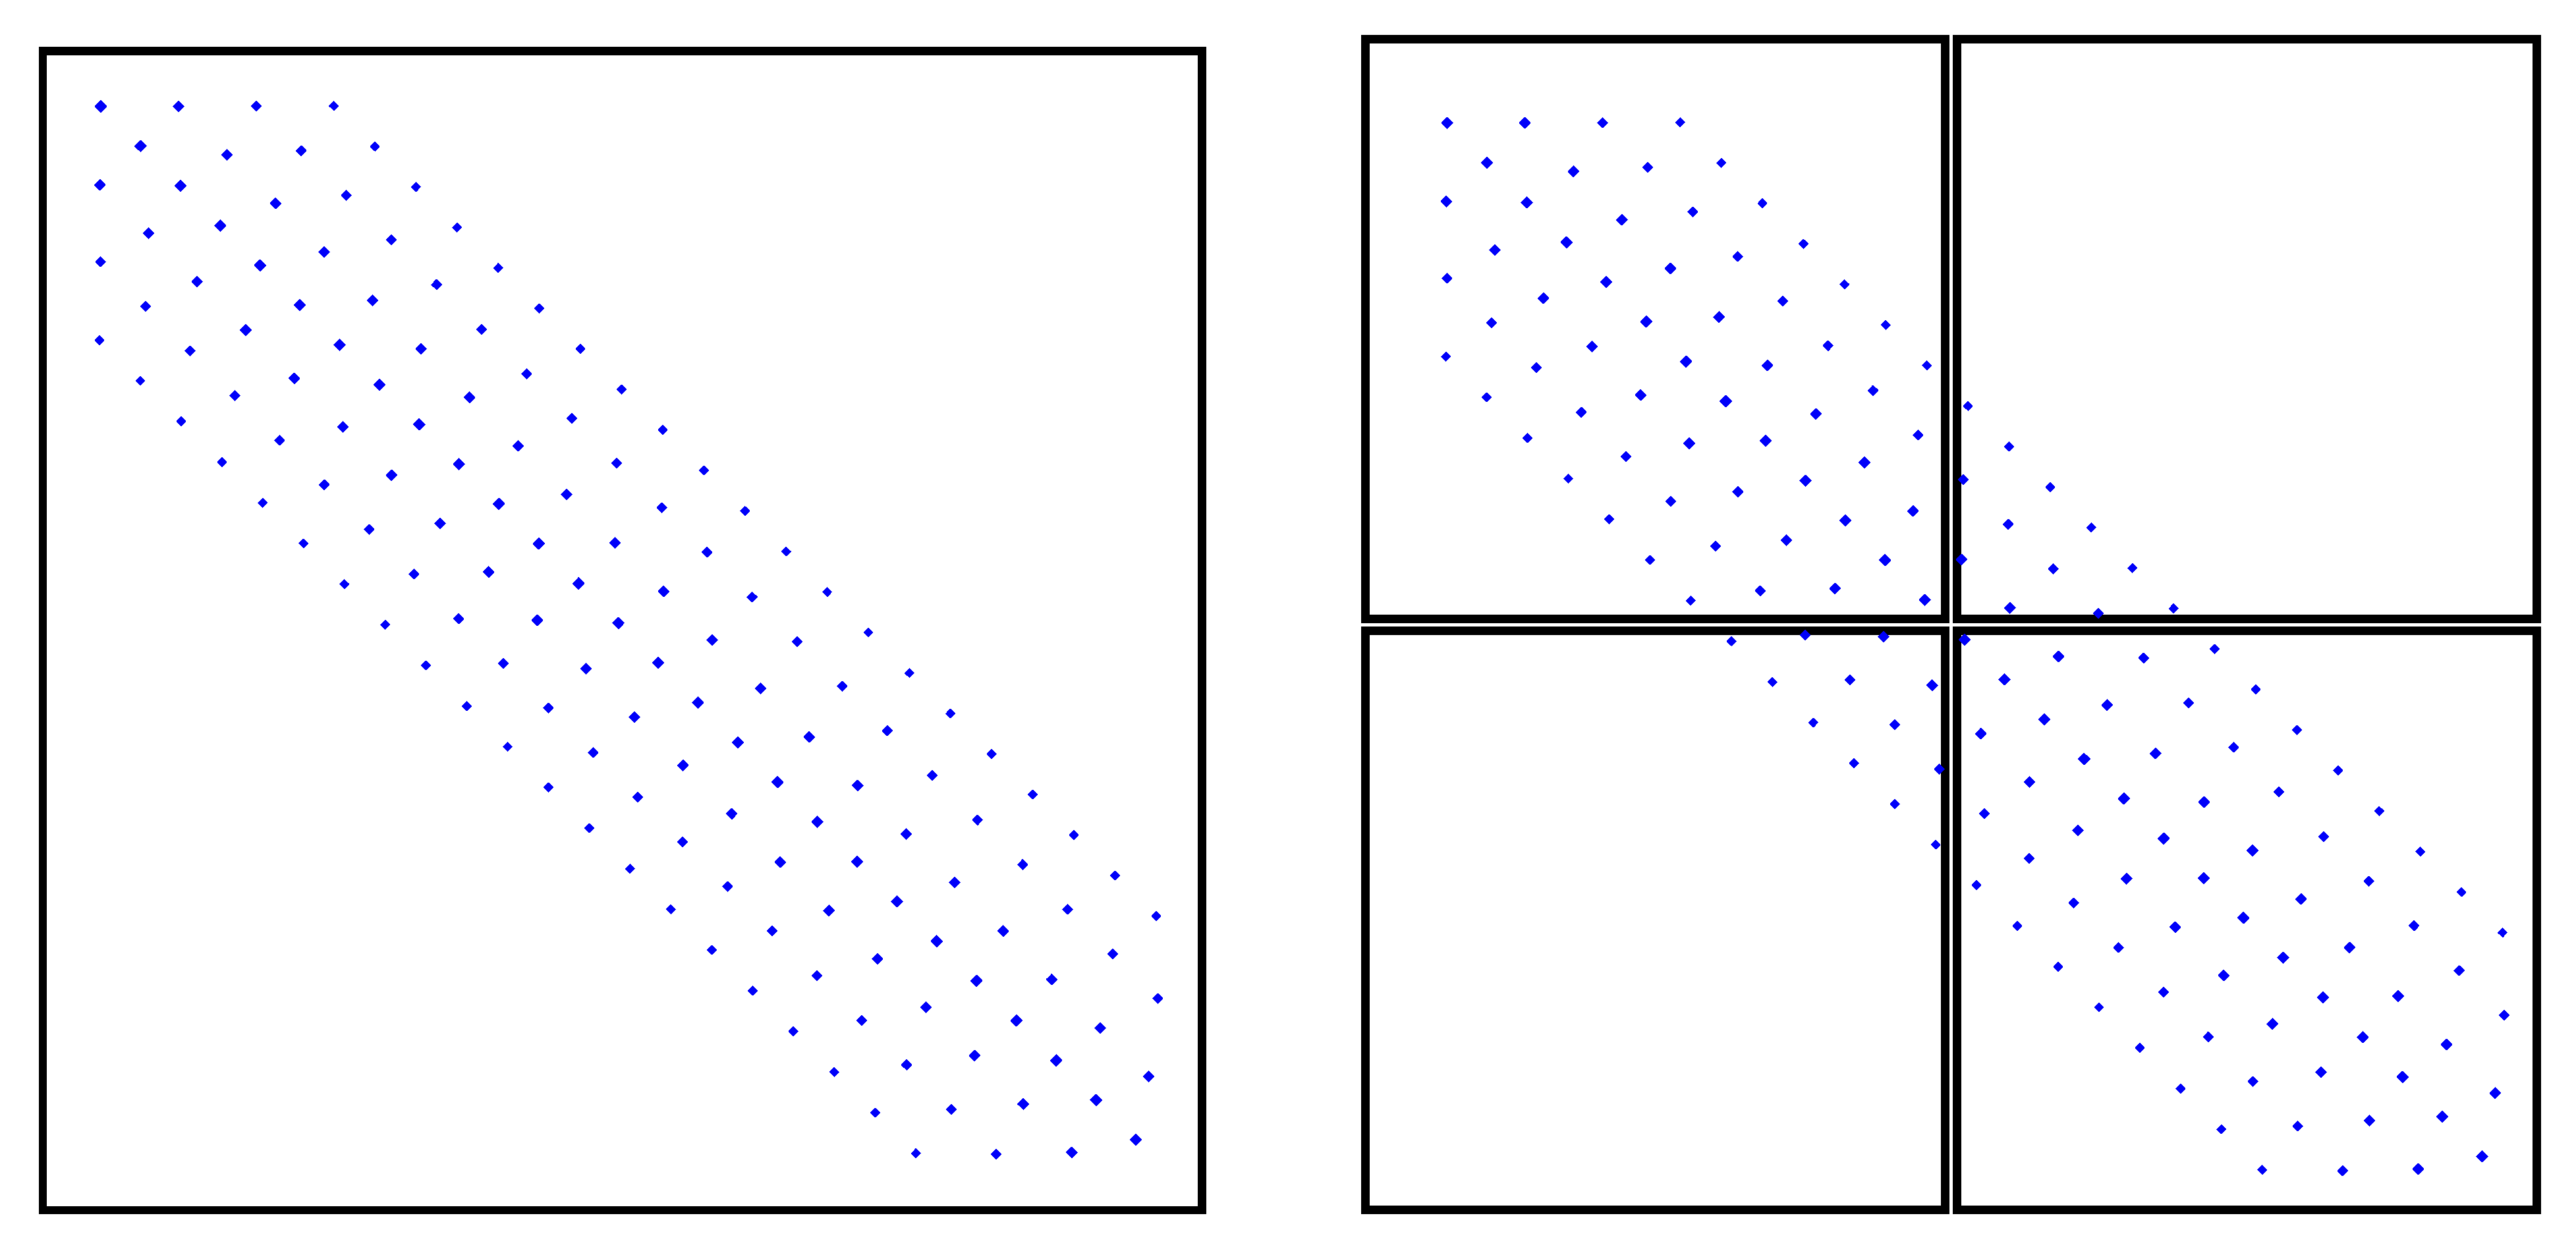
\includegraphics[width=8.5cm,height=4cm]{./figures/split3.pdf}
 \caption{Using row and column sizes to decide when to stop the recursion is not efficient, because the top left block is the same size as the top right one, but it should be divided to more sub-blocks.}
 \label{fig:thres}
 \Description{}
\end{figure}

Furthermore, by splitting sparse matrices recursively, we will have more and more zero rows and columns in the resulting blocks. So, using row size and column size of the blocks is not very helpful. Instead, we use nonzero rows and nonzero columns.

At the start of the recursive function, the number of nonzero rows of A ($A\_nnz\_row$) and nonzero columns of B ($B\_nnz\_col$) are being computed. A threshold for 
\begin{equation}
    \nnzsz = A\_nnz\_row \times B\_nnz\_col
\end{equation}

is set. Our algorithm has a profiling step where it empirically determines the appropriate threshold by running several test cases. On the machines we used,  $20M$ was chosen as the threshold. We continue splitting the matrices until the threshold is reached, and then we preform the multiplication.

%First method uses a dense matrix.
%The matrices are ordered as column-major.
% In the first method, a dense matrix of size $\nnzsz$ is initialized to $0$. \mr{explain better:}Each nonzero of $B$ is multiplied by its corresponding nonzero of $A$ and the result will be added to the corresponding index in the dense matrix. At the end, we go through the dense matrix and add the nonzeros to the final multiplication matrix.

We have implemented two methods to perform the multiplication: 
\begin{enumerate}
    \item dense buffer
    \item hashmap
\end{enumerate}

When performing the multiplication, at least one of the matrices, typically the output, needs random access as it is accumulating the results. Given that the divide and conquer approach has reduced the size of the output matrix, the first approach is to keep a temporary buffer for dense matrix storage. Each nonzero of $B$ is multiplied by its corresponding nonzero of $A$ and the result will be added to the corresponding index in the dense matrix. As long as the dense matrix is small enough to fit within the L2 cache, we should get good performance. At the end of the multiplication, we traverse the dense matrix and extract the non-zeros as a sparse matrix. This approach works well as long as the resulting matrix is dense. We allocate a memory block of size of the threshold before starting the matrix product. When we reach the stop condition for each recursive call, we preform the following steps:
\begin{enumerate}
    \item Initialize the first \nnzsz~ entries to 0.
    \item Perform the multiplication and add the result entries to the buffer matrix.
    \item Extract nonzeros from the dense matrix and add them to C.
\end{enumerate}

When the ratio of nonzeros to \nnzsz~ is low, it becomes inefficient to traverse the whole dense matrix and check for nonzeros in the final stage. To solve this issue, we use an efficient hashmap to achieve similar results without the $\mathcal{O}(n^2)$ overhead of extracting the non-zeros from the dense matrix. The entry's index is the key and its value is the hashmap's value. When we want to add the multiplication of nonzeros of $A$ and $B$ to the hashmap, we check if the index exists in the map. If it exists the value is being added to the existing one's. Otherwise a new entry will be added to the hashmap. Clearly, there is an overhead to this approach that needs to be balanced against the overheads associated with the dense representation. 

To measure of the effectiveness of our method in a practical situation, we have implemented the \recmm~ function in our Algebraic Multigrid solver, called \textit{Saena}, and performed \mm~ twice to compute the coarse matrix based on the 3D Poisson Problem.

In Figure~\ref{fig:lap60}, we compare the two methods for computing coarse matrix $Ac = R \times A \times P$, in which $A$ is the 3D Poisson problem of size $216k$. For $0 \leq \nnzsz \leq 10M$, in $1M$ steps, we compare the two methods in order to develop an efficient hybrid algorithm. For instance, the first point indicates that the dense structure is better than the hashmap approach in $1245$ cases for the multiplications such that $0 \le\ \nnzsz < 1M$. For the lower range the dense representation is better and for the higher range the hashmap is significantly faster. Figure~\ref{fig:eco} shows the same experiment for matrix ID $1882$ from SuiteSparse (Florida) Matrix Collection, which is a sparse matrix of size $1M$ and $5M$ nonzero.

\begin{figure}[tbh]
 \centering
 %\Description{Description}
 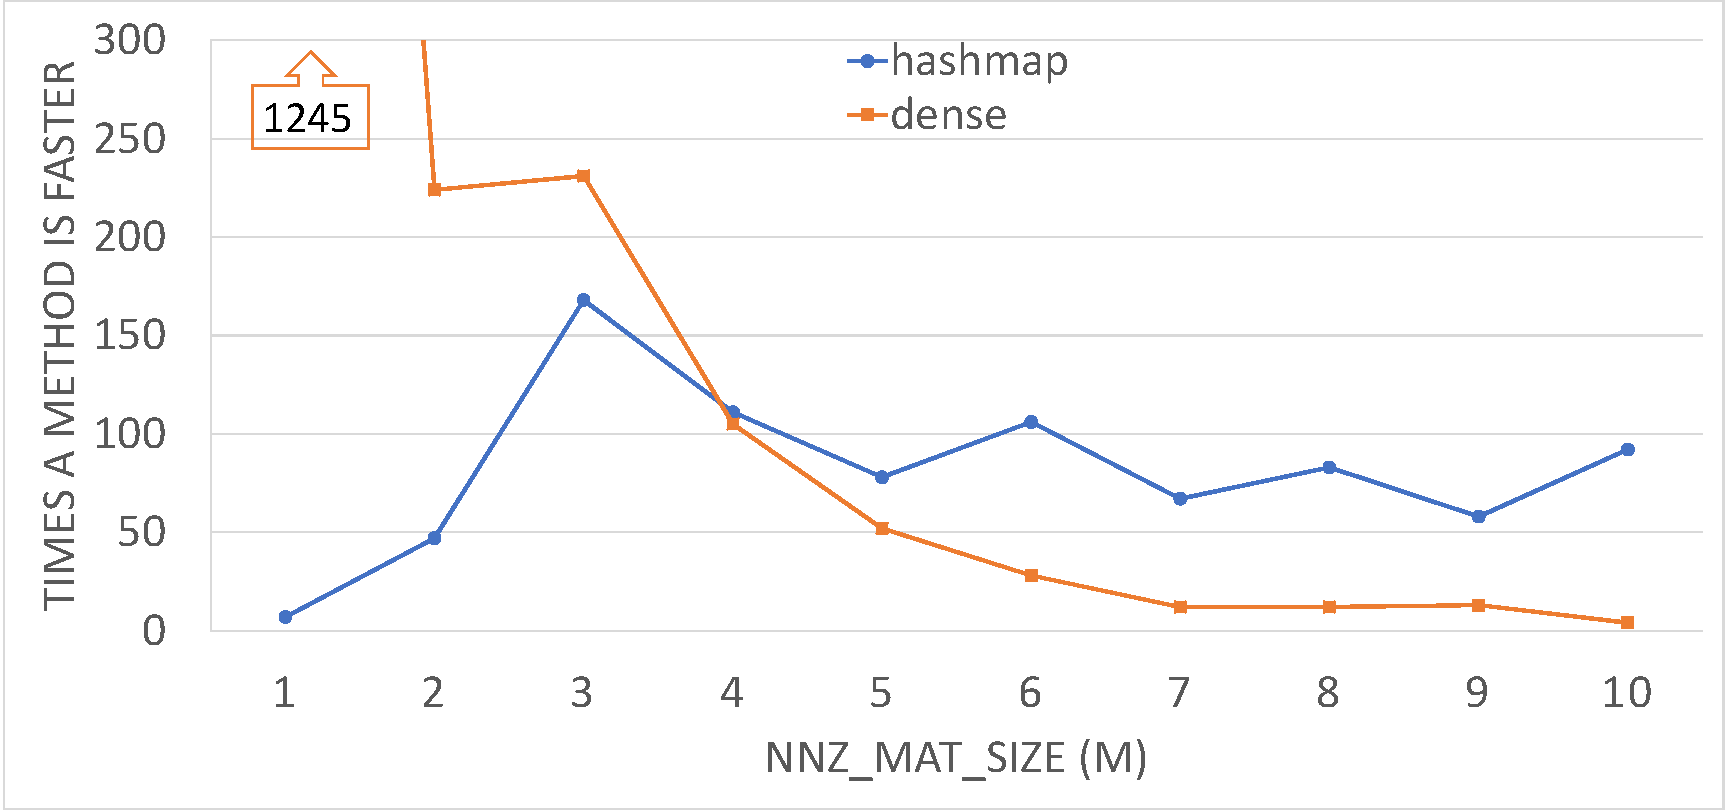
\includegraphics[width=8.5cm,height=4cm]{./figures/lap60_range.pdf}
 \caption{Comparison between dense structure method with hashmap to compute coarse matrix $Ac = R \times A \times P$, in which $A$ is the 3D Poisson problem of size $216k$. The plot shows the number of times each method is faster than the other one in intervals of $1M$ for $\nnzsz$.}
 \label{fig:lap60}
 \Description{}
\end{figure}

A combination of these two methods would give us the best performance across different matrix structures and densities. The dense method is being used for the lower range and the hashmap for the higher range.
We have done a series of experiments to determine the threshold when to switch between the two methods. Figures~\ref{fig:lap60} and \ref{fig:eco} suggest to use the dense structure method when $0 \le\ \nnzsz < 4M$ and use hashmap for the rest. We noticed that when hashmaps are better, the difference time between the two methods on average is higher. In other words, on average, $n$ times performing hashmap is faster than $n$ times using the dense structure. So empirically, we found $1M$ to be a good estimate for switching between the two methods.

\begin{figure}[tbh]
 \centering
%\Description{Description}
 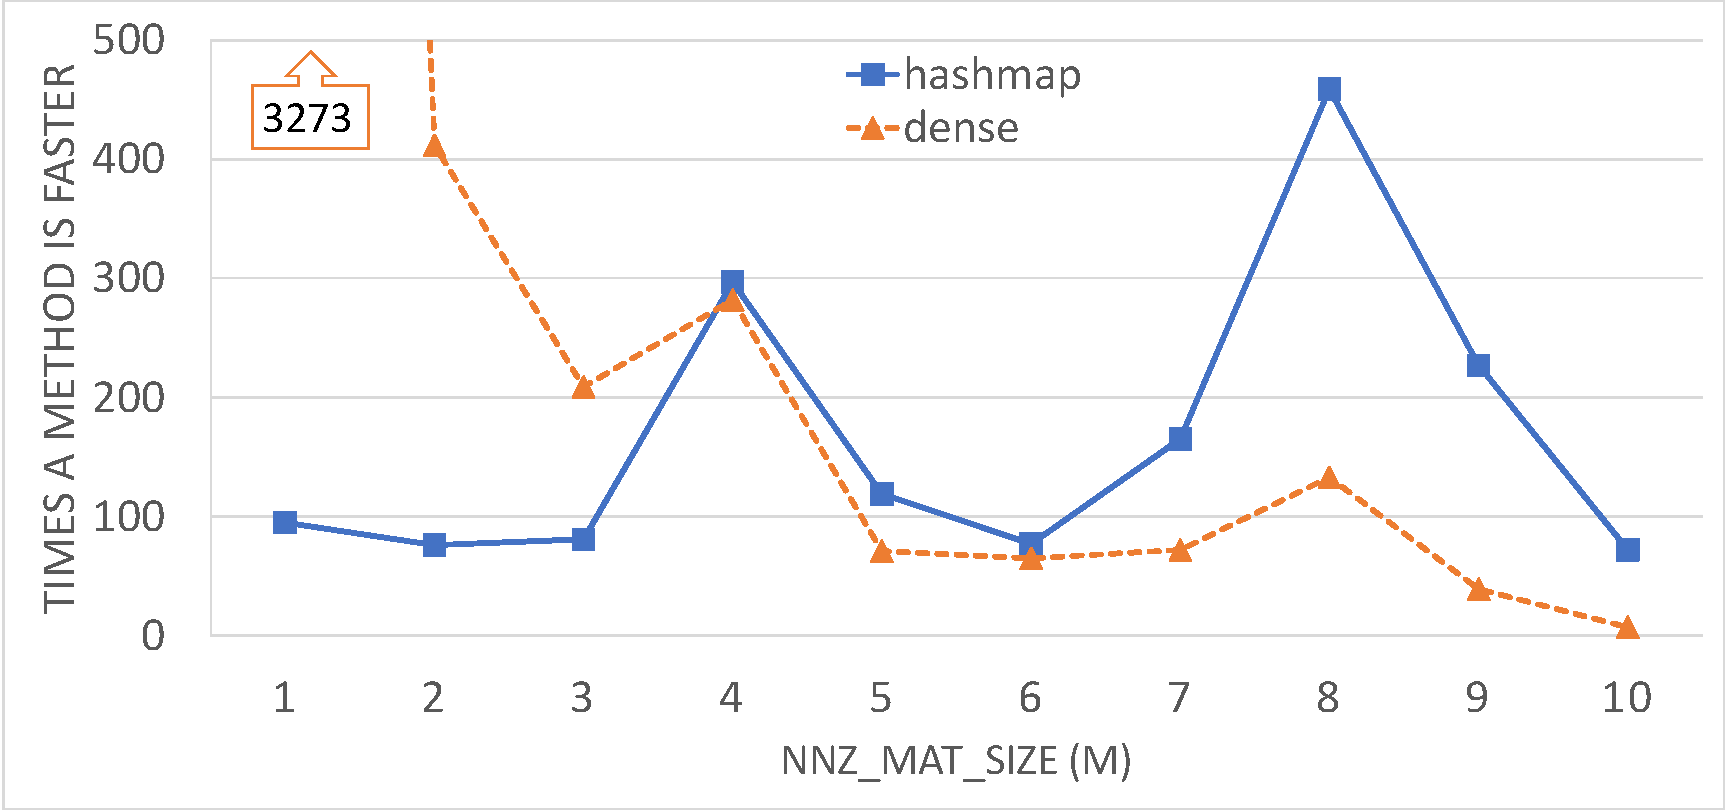
\includegraphics[width=8.5cm,height=4cm]{./figures/eco_range.pdf}
 \caption{Comparison between dense structure method with hashmap to compute coarse matrix $Ac = R \times A \times P$, in which $A$ is matrix ID $1882$ from SuiteSparse (Florida) Matrix Collection. The plot shows the number of times each method is faster than the other one in intervals of $1M$ for $\nnzsz$.}
 \label{fig:eco}
 \Description{}
\end{figure}

\begin{figure}[tbh]
 \centering
 %\Description{Description}
 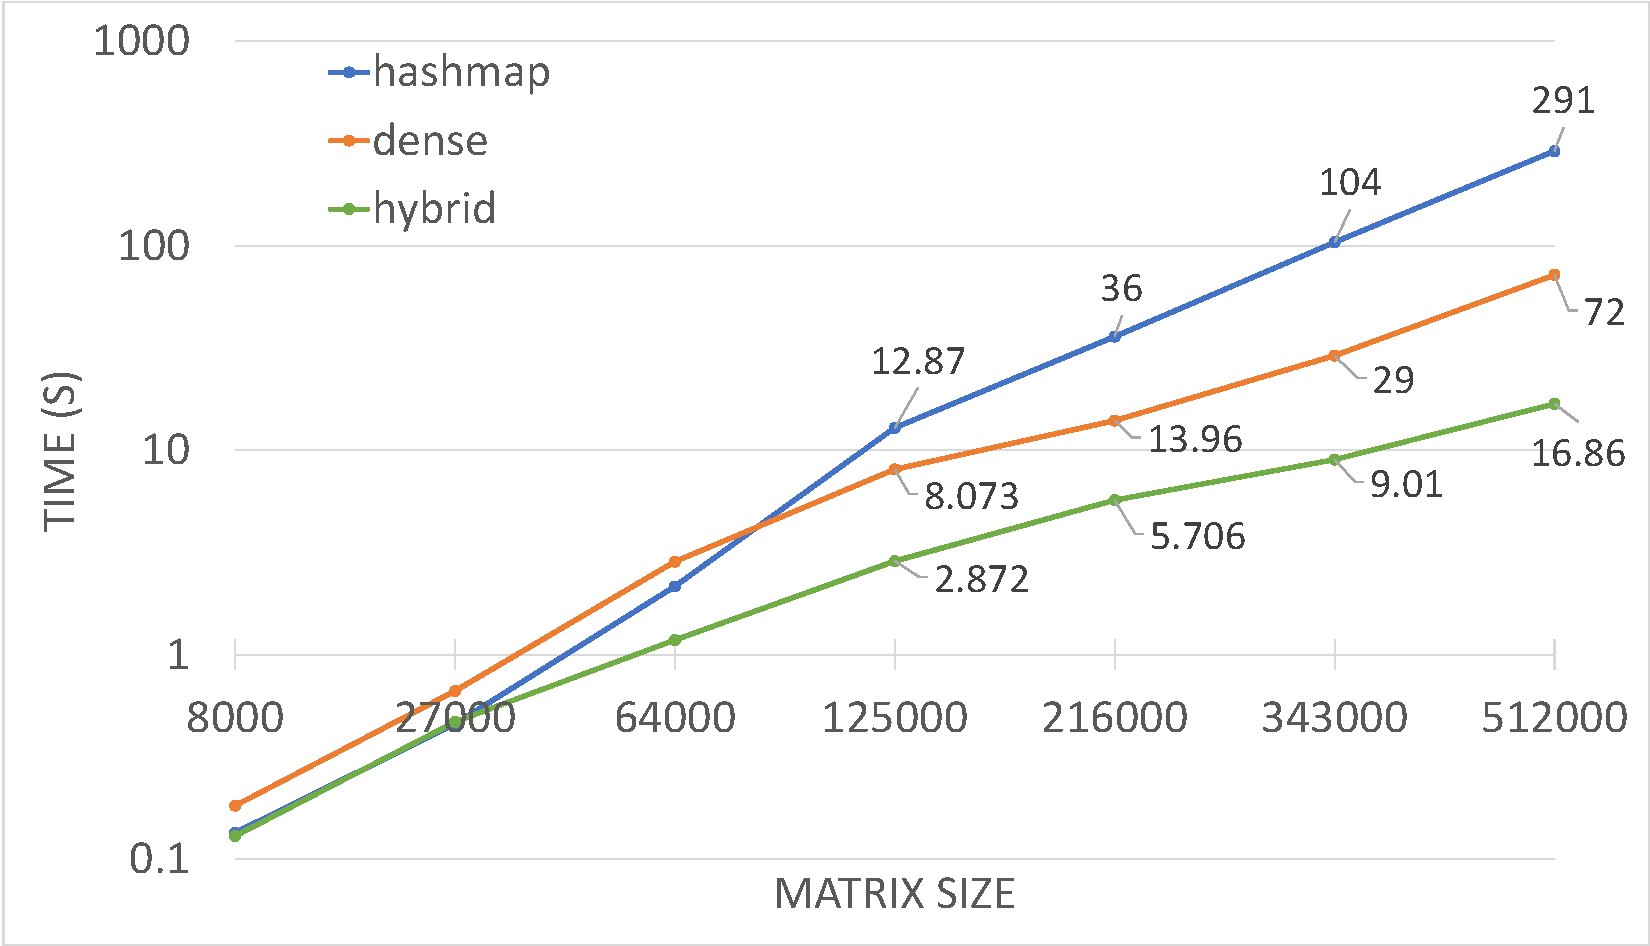
\includegraphics[width=8.5cm,height=5cm]{./figures/mix.pdf}
 \caption{Comparison between the three methods to do Case 1: only using hashmap, only using the dense structure, and the hybrid method. They are used as Case 1 to compute the first coarse matrix (the triple multiplication) on 7 matrices (3D Poisson) of different sizes.}
 \label{fig:mix}
 \Description{}
\end{figure}

Figure~\ref{fig:mix} compares the hybrid method with the basic two methods. We have compared the three approaches on different sizes of 3D Poisson problem, ranging from $8k$ to almost half a million. For instance, for the case where the matrix is of size $512k$, performing the triple matrix product takes $291s$ if only hashmap is used for Case 1, takes $72s$ if only the dense structure is used and finally takes almost $17s$ when the hybrid approach is utilized.


\subsubsection{Case 2}
\label{sec:case2}
When A is horizontal, i.e. its row size is less than or equal to its column size, we halve A by column based on its column size (Figure~\ref{fig:case2_left}). Since row size of B equals column size of A, we halve B by row, so it will be a split similar to A, but horizontally.
Then, the \recmm~ will be called twice, once on $A1$ and $B1$, and again on $A2$ and $B2$ (Algorithm~\ref{alg:case2}). The results of the two multiplications need to be added together at the end. It means, there will be entries for the result matrix with the same index. We call these entries \textit{duplicates}. Since there will be numerous nested recursive calls, we avoid doing adding duplicates at this stage. After the first recursive function is finished, we will perform a sorting and then add the duplicates only once at the end.

\begin{figure}[tbh]
    \centering
    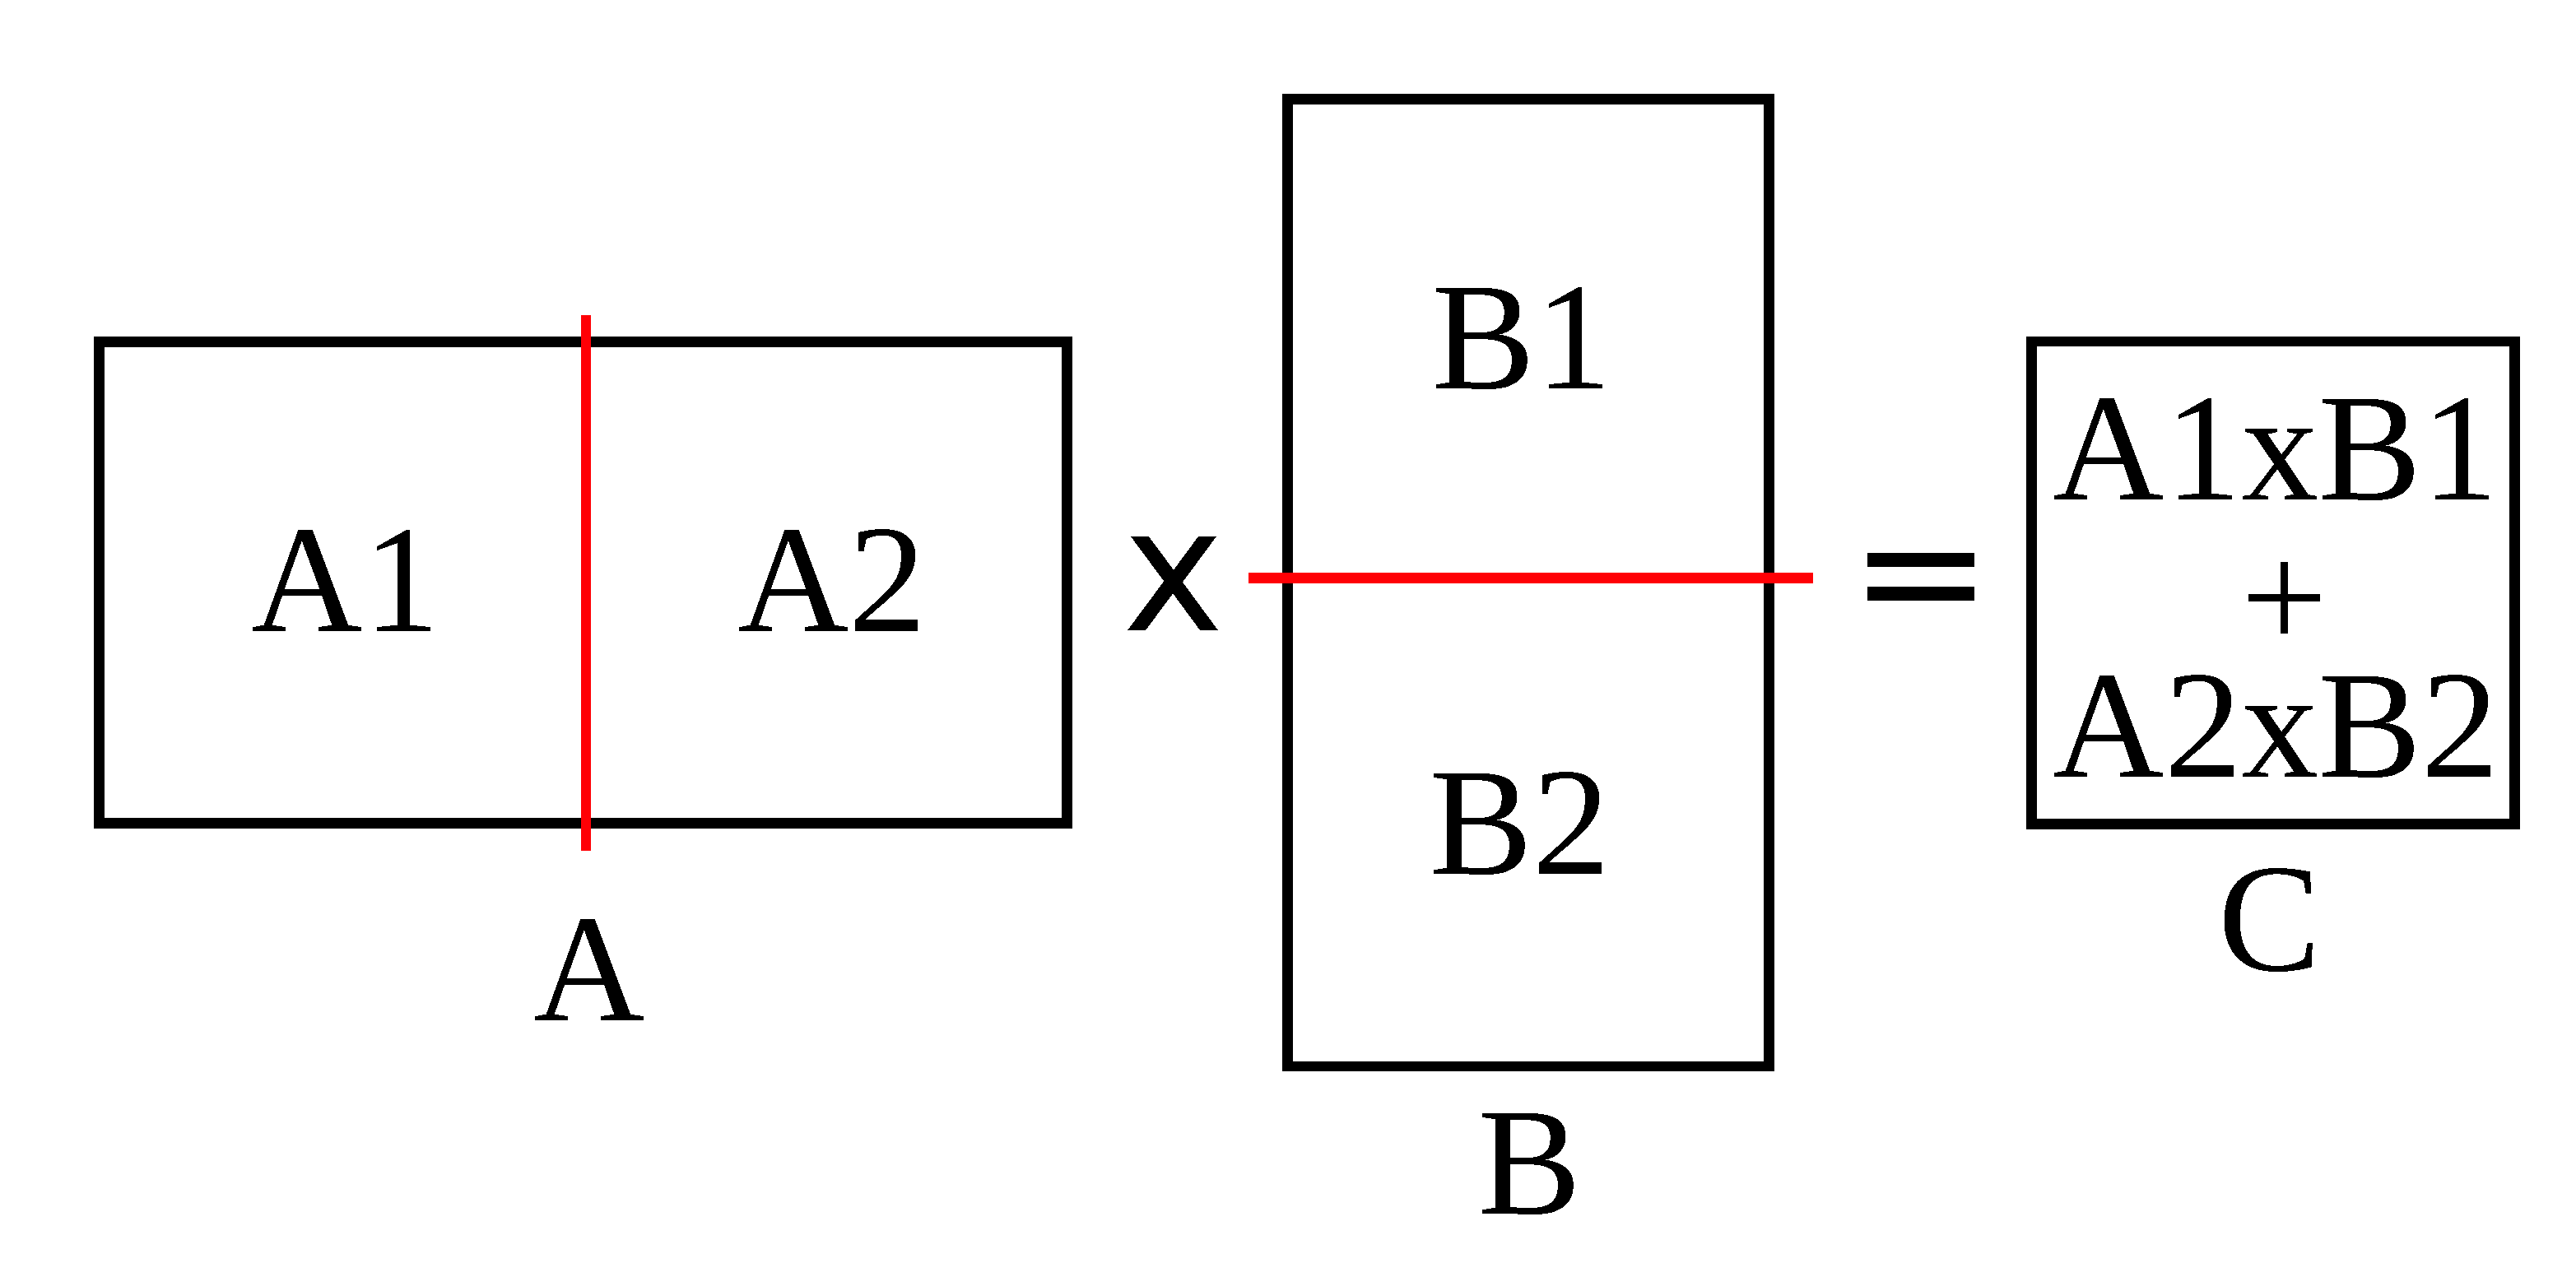
\includegraphics[width=4.5cm,height=2.3cm]{./figures/case2_001.pdf}
    \caption{Case 2: When A is horizontal, split A by column and B by row. Call the recursive function twice.}
    \label{fig:case2_left}
    \Description{}
\end{figure}

\begin{figure}[tbh]
    \centering
    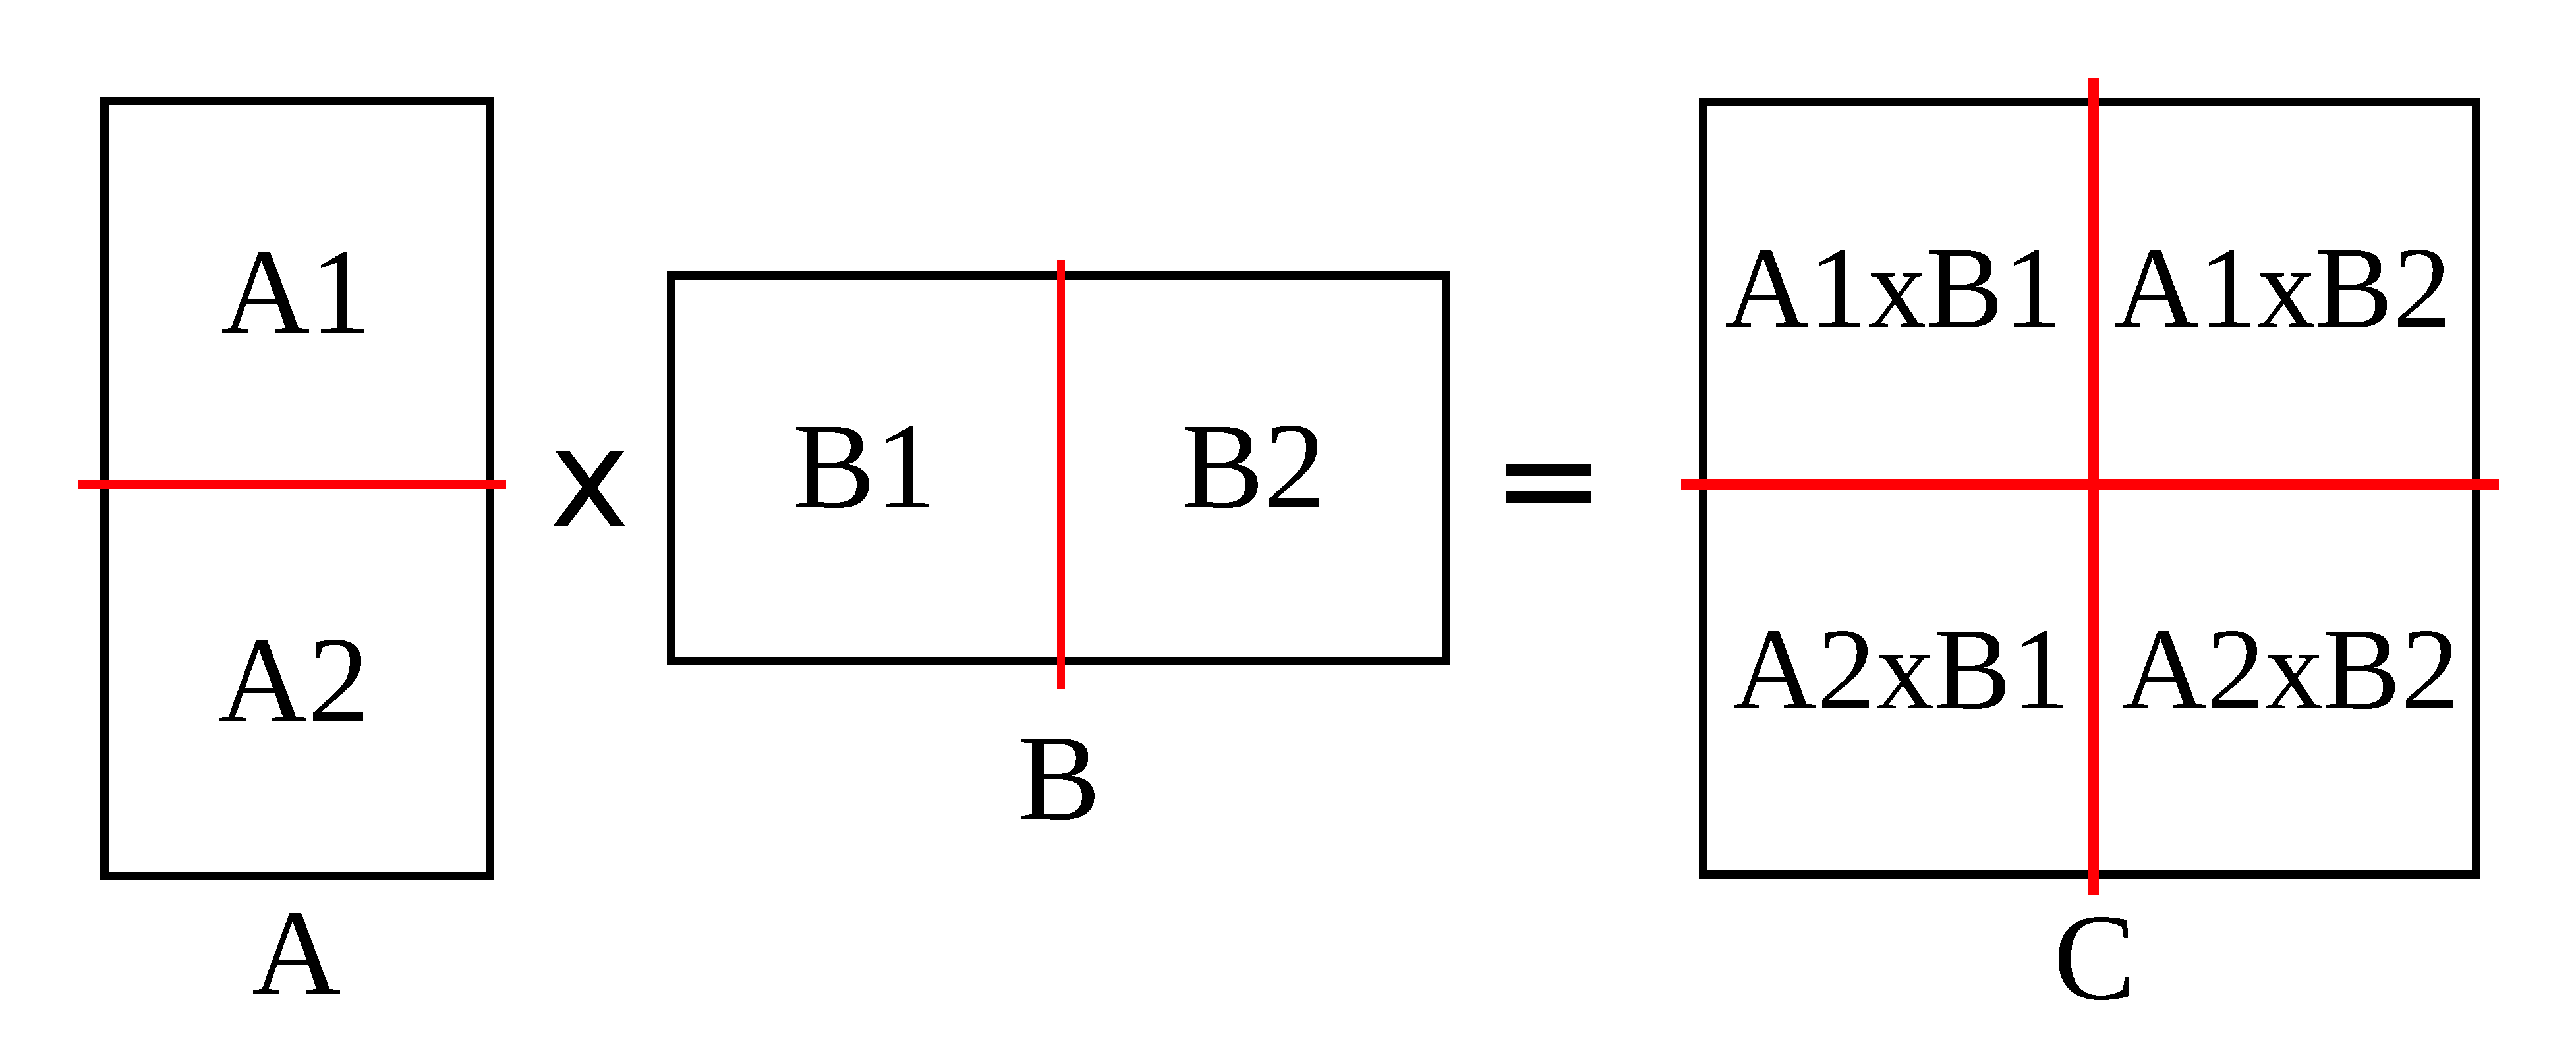
\includegraphics[width=5.5cm,height=2.3cm]{./figures/case3_001.pdf}
    \caption{Case 3: When A is vertical, split A by row and B by column. Call the recursive function four times.}
    \label{fig:case3}
    \Description{}
\end{figure}

\begin{algorithm}[tbh] 
  %\footnotesize
  \caption{Case 2: $C = \recmm2(A, B)$} 
  \begin{algorithmic}[1]
    \Require $A$, $B$
    \Ensure  $C$
    \State $(A1, A2) = \spc(A)$
    \State $(B1, B2) = \spr(B)$
    \State $C \leftarrow \recmm(A1,B1)$
    \State $C \leftarrow \recmm(A2,B2)$
    %\State $C \leftarrow \textsc{mergesort}(C1, C2)$
  \end{algorithmic}
  \label{alg:case2}
  \Description{}
\end{algorithm}

\subsubsection{Case 3}
\label{sec:case3}
When A is vertical, i.e. its row size is greater than its column size, we halve A by row based on its row size and halve B by column (Figure~\ref{fig:case3}). In contrary to the previous case, the column size of B is not related to row size of A, so they are split independently. This time the \recmm~ will be called four times (Algorithm~\ref{alg:case3}).  Although we have 4 recursive calls in this case, but there is no duplicates at the end, which makes this case more efficient than Case 2 for the total time, because it is faster to do the sorting and adding duplicates at the end on a smaller set of entries. 

\iffalse
\begin{figure}[tbh]
 \centering
 %\Description{Description}
 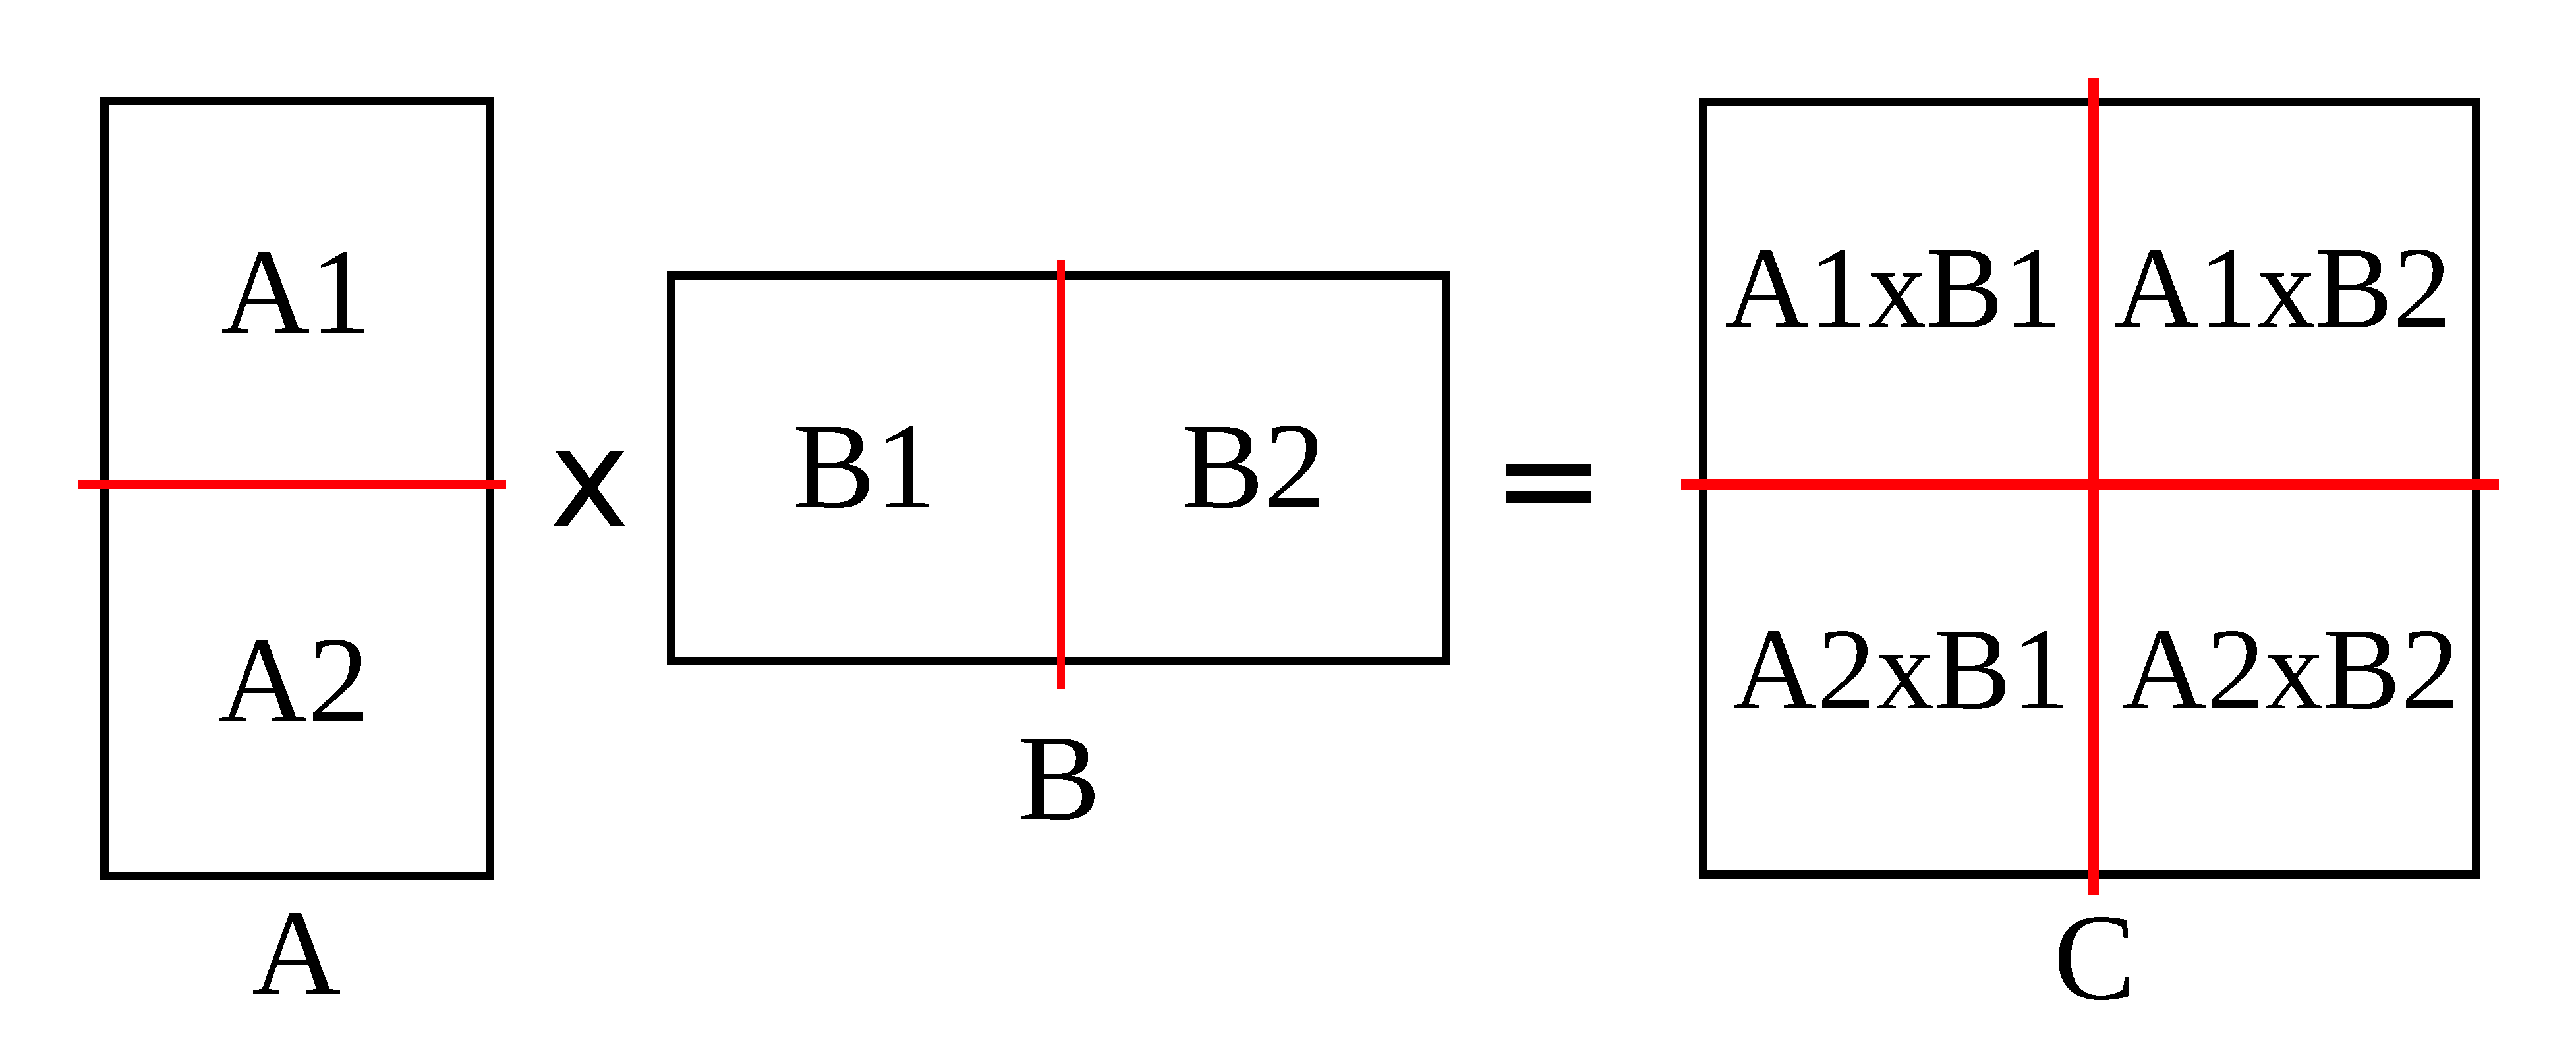
\includegraphics[width=6cm,height=2.5cm]{./figures/case3_001.pdf}
 \caption{Case 3: When A is vertical, split A by row and B by column. Call the recursive function four times.}
 \label{fig:case3}
\end{figure}
\fi

\begin{algorithm}[H] 
  %\footnotesize
  \caption{Case 3: $C = \recmm3(A, B)$} \label{alg:case3} 
  \begin{algorithmic}[1]
    \Require $A$, $B$
    \Ensure  $C$
    \State $(A1, A2) = \spr(A)$
    \State $(B1, B2) = \spc(B)$
    \State $C \leftarrow \recmm(A1,B1)$
    \State $C \leftarrow \recmm(A2,B1)$
    \State $C \leftarrow \recmm(A1,B2)$
    \State $C \leftarrow \recmm(A2,B2)$
    %\State $\textsc{sort}(C)$
  \end{algorithmic}
  \label{alg:case3}
\end{algorithm}

We have also implemented splitting based on the number of nonzeros. In \textit{Case 2}, we split $A$ in a way to have half of nonzeros in $A1$, and the other half in $A2$. The same split is used for $B$. In \textit{Case 3}, we do the same, but separately for both $A$ and $B$. After a series of experiments we noticed that the splitting method based on size scales better than splitting based on nonzeros.

\subsubsection{All together}

When all three cases work together, we have Case 2 and Case 3, that aim to divide the matrices into skinny matrices such that the resulting matrix is small. Then by using a hybrid multiplication algorithm, we get these results. These results are then accumulated and merged together. From a memory access perspective, the accumulation and merging required for Case 2 and 3 is structured access to the matrix, with the only random access happening during Case 1. This makes the overall algorithm very efficient. 

\subsection{Communication}
\label{sec:amg}

In the previous section we explained how to perform \mm~ if the data is available locally. In this section, we explain how the communication is done to perform
\begin{equation}
    C = A \times B
\end{equation}
in a distributed fashion for general (non necessarily symmetric) matrices $A$ and $B$. Also, we show how to improve performance and scalability if $B$ is symmetric.

Matrices are partitioned across multiple processors by row blocks (Figure~\ref{fig:partition}). Matrices $A$ and $P$ have the same number of rows and consequently are partitioned the same way. $R$ has fewer number of rows and has a different partition. This is because coarsening need not be uniform across processes. Consequently the partitioning of the rows of $R$ could be different from that of $A$ and $P$. The triple matrix product is performed in two parts: first $A \times P$ is computed, followed by $R \times B$, where $B = A \times P$ is the result of the first multiplication. In other words, this is equivalent to performing matrix-matrix multiplications (\mm) twice.

\begin{figure}[tbh]
 \centering
 %\Description{Description}
 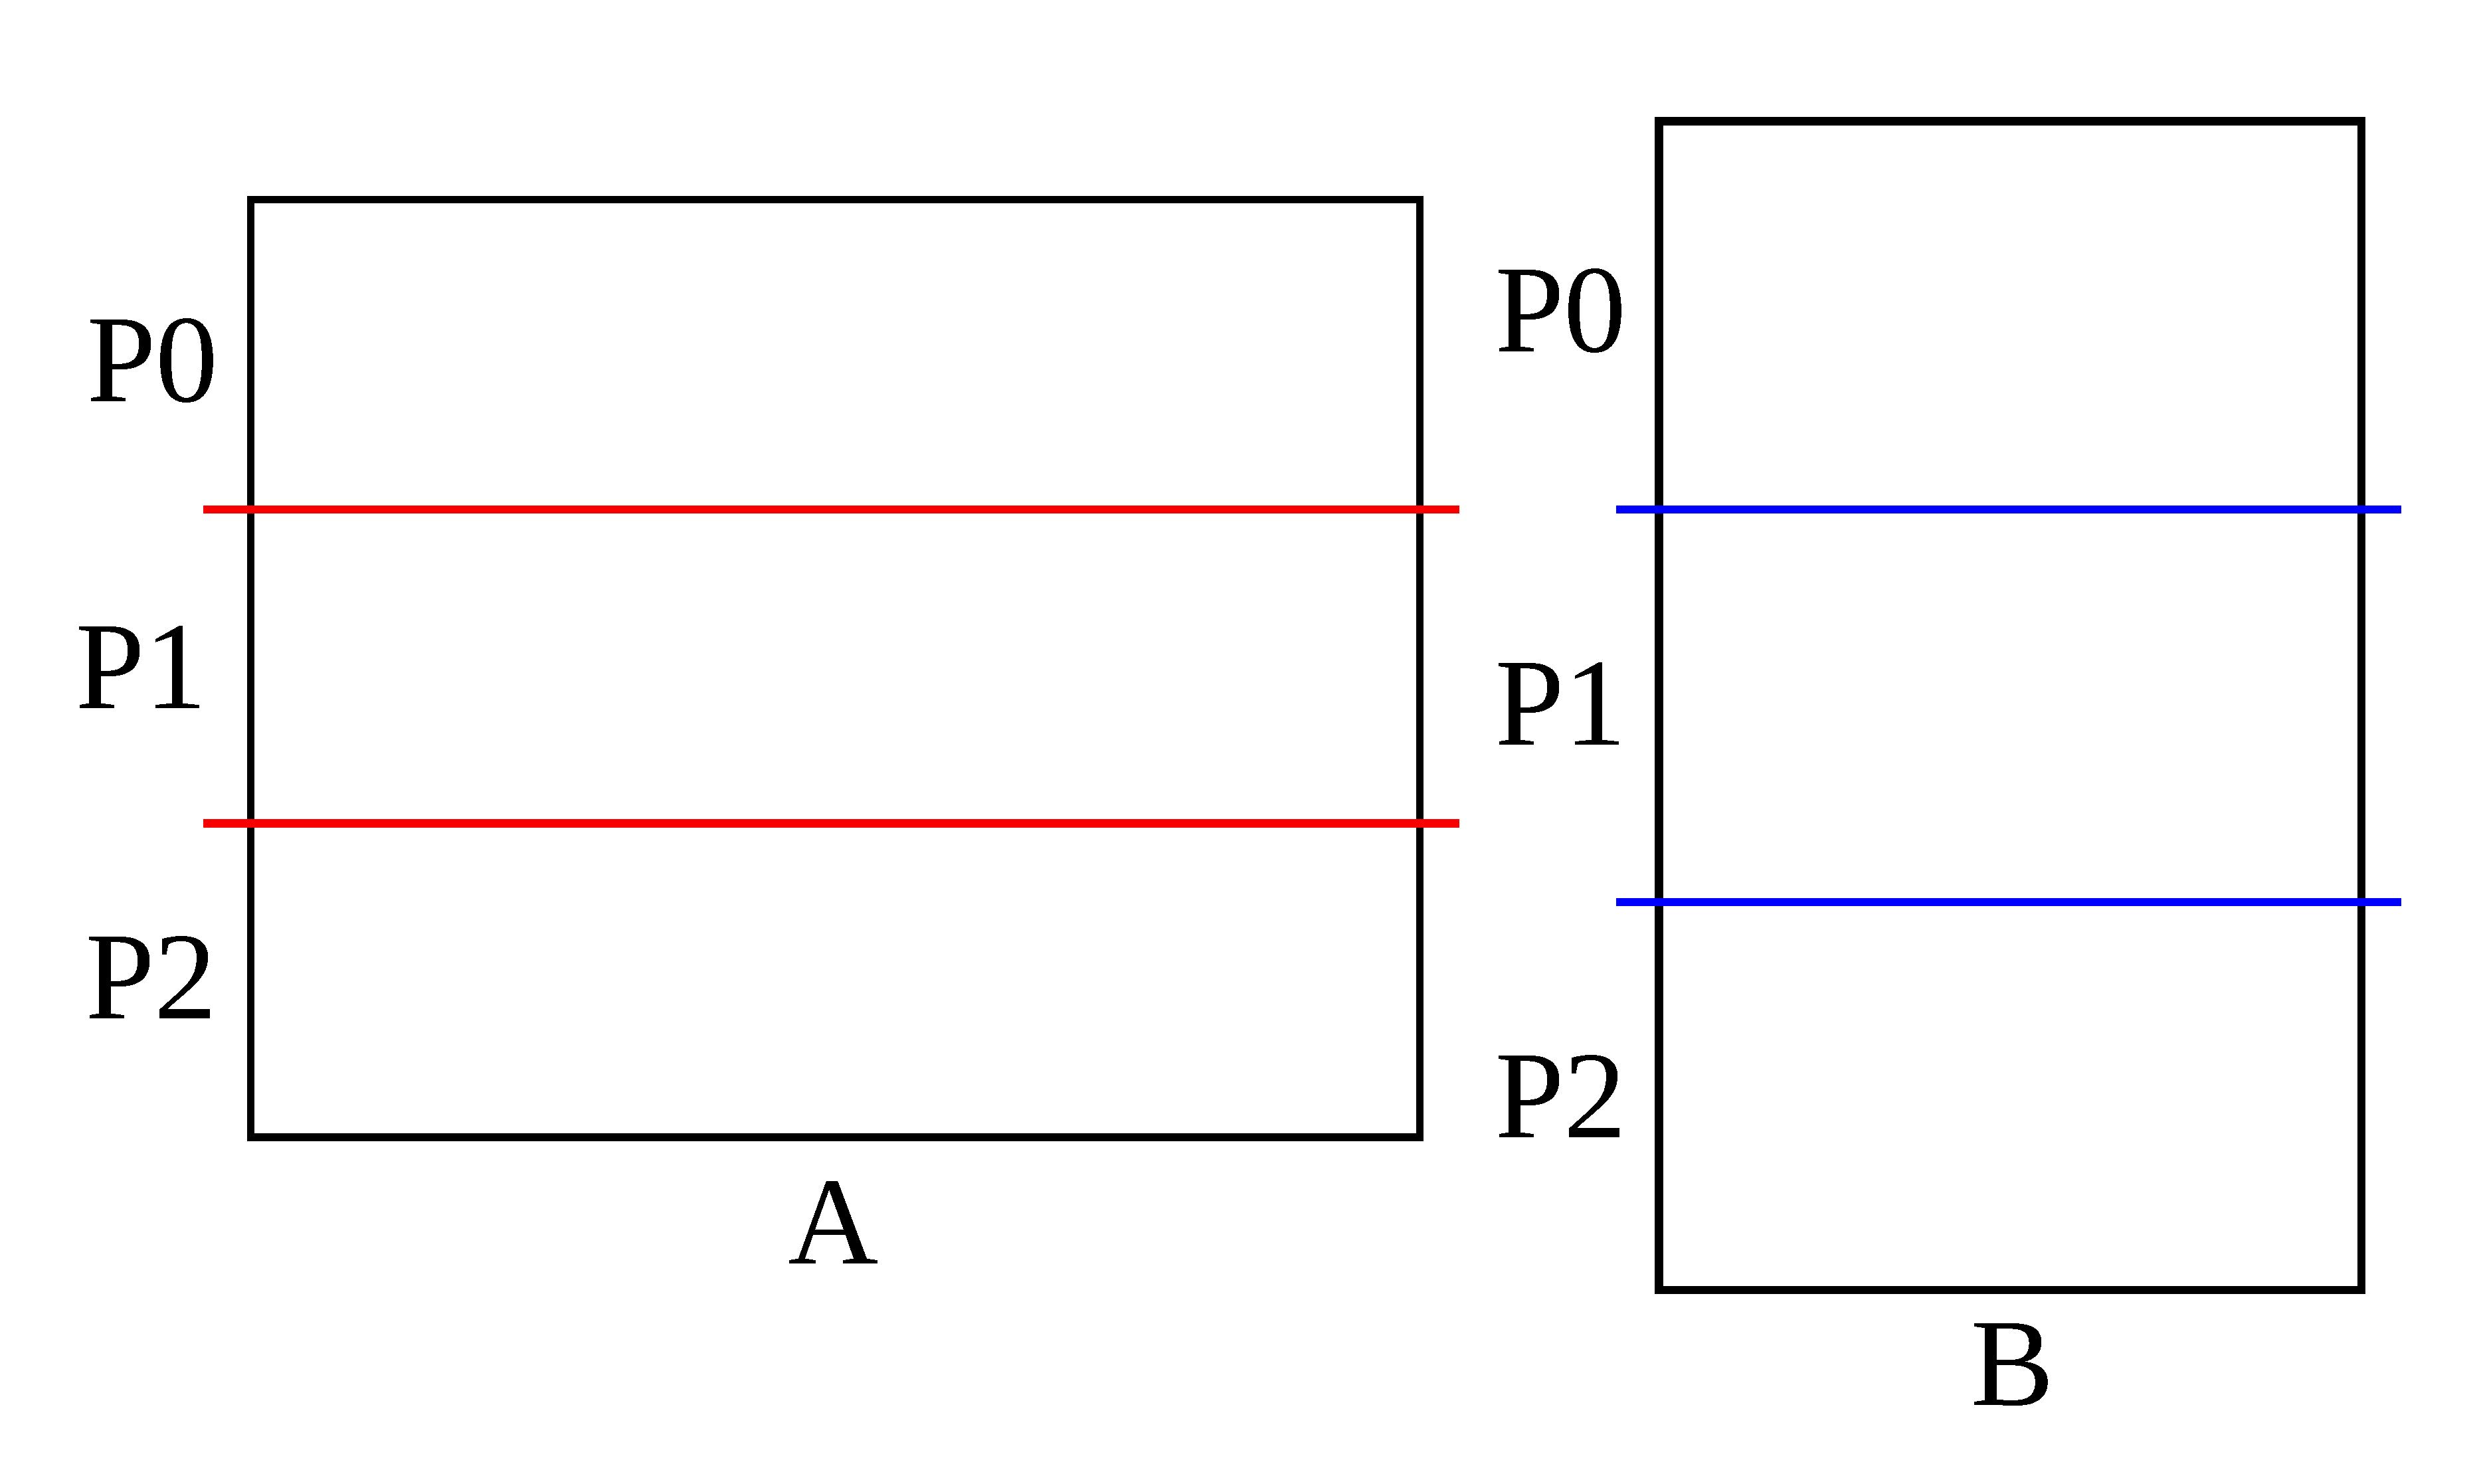
\includegraphics[width=5.3cm,height=2.8cm]{./figures/partition2.pdf}
 \caption{Partitioning of the matrices across the processors in row blocks.}
 \label{fig:partition}
 \Description{}
\end{figure}

Now, we explain how to compute $B := A \times P$. We assume the same partition of rows of $A$ on also its columns (red lines) since $A$ is square. For columns of $P$ we use the partition of rows of $R$ (blue lines in Figure~\ref{fig:part1b}).
Without loss of generality, let us focus on how to perform \mm ~on processor $P1$. To compute entry $B(i, j)$, we need to multiply row $i$ of $A$ with column $j$ of $P$ and add them together (since we are working with sparse matrices, we only consider the nonzeros here).

\begin{figure}[tbh]
    \centering
    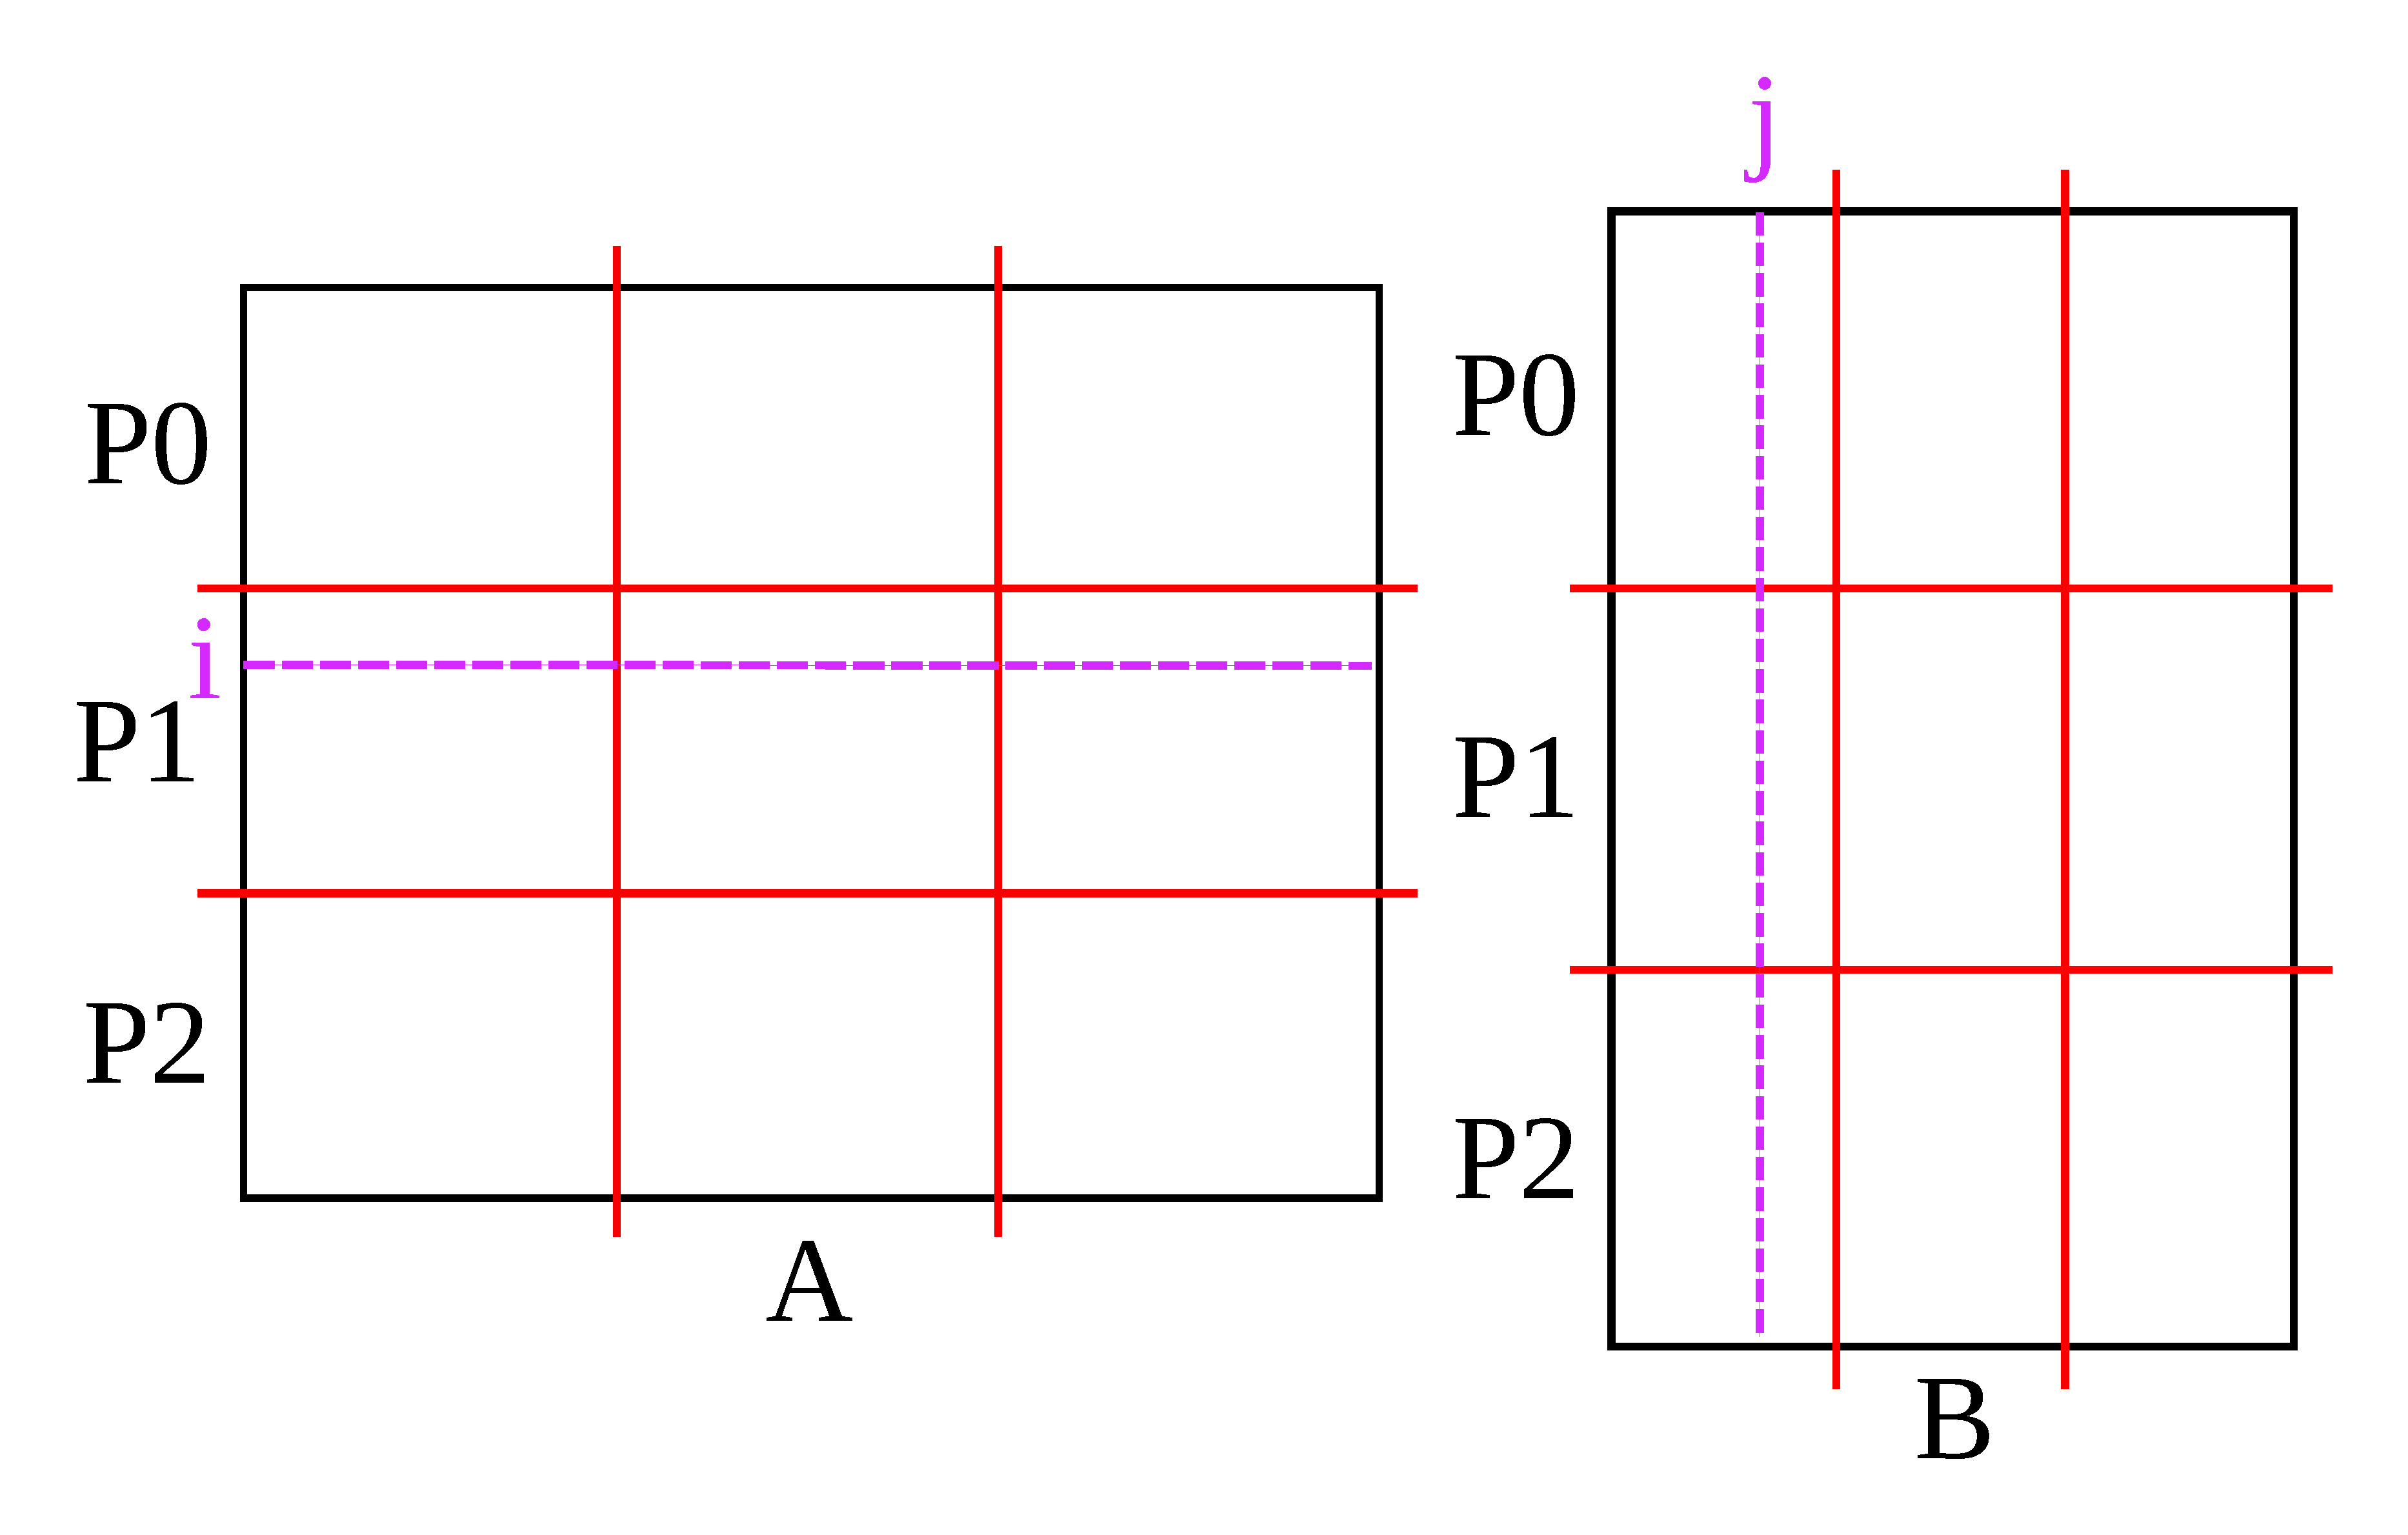
\includegraphics[width=5cm,height=3cm]{./figures/partition3.pdf}
    \caption{Column $j$ of $B$ is stored on different processors.}
    \label{fig:part1b}
    \Description{}
\end{figure}

\begin{figure}[tbh]
    \centering
    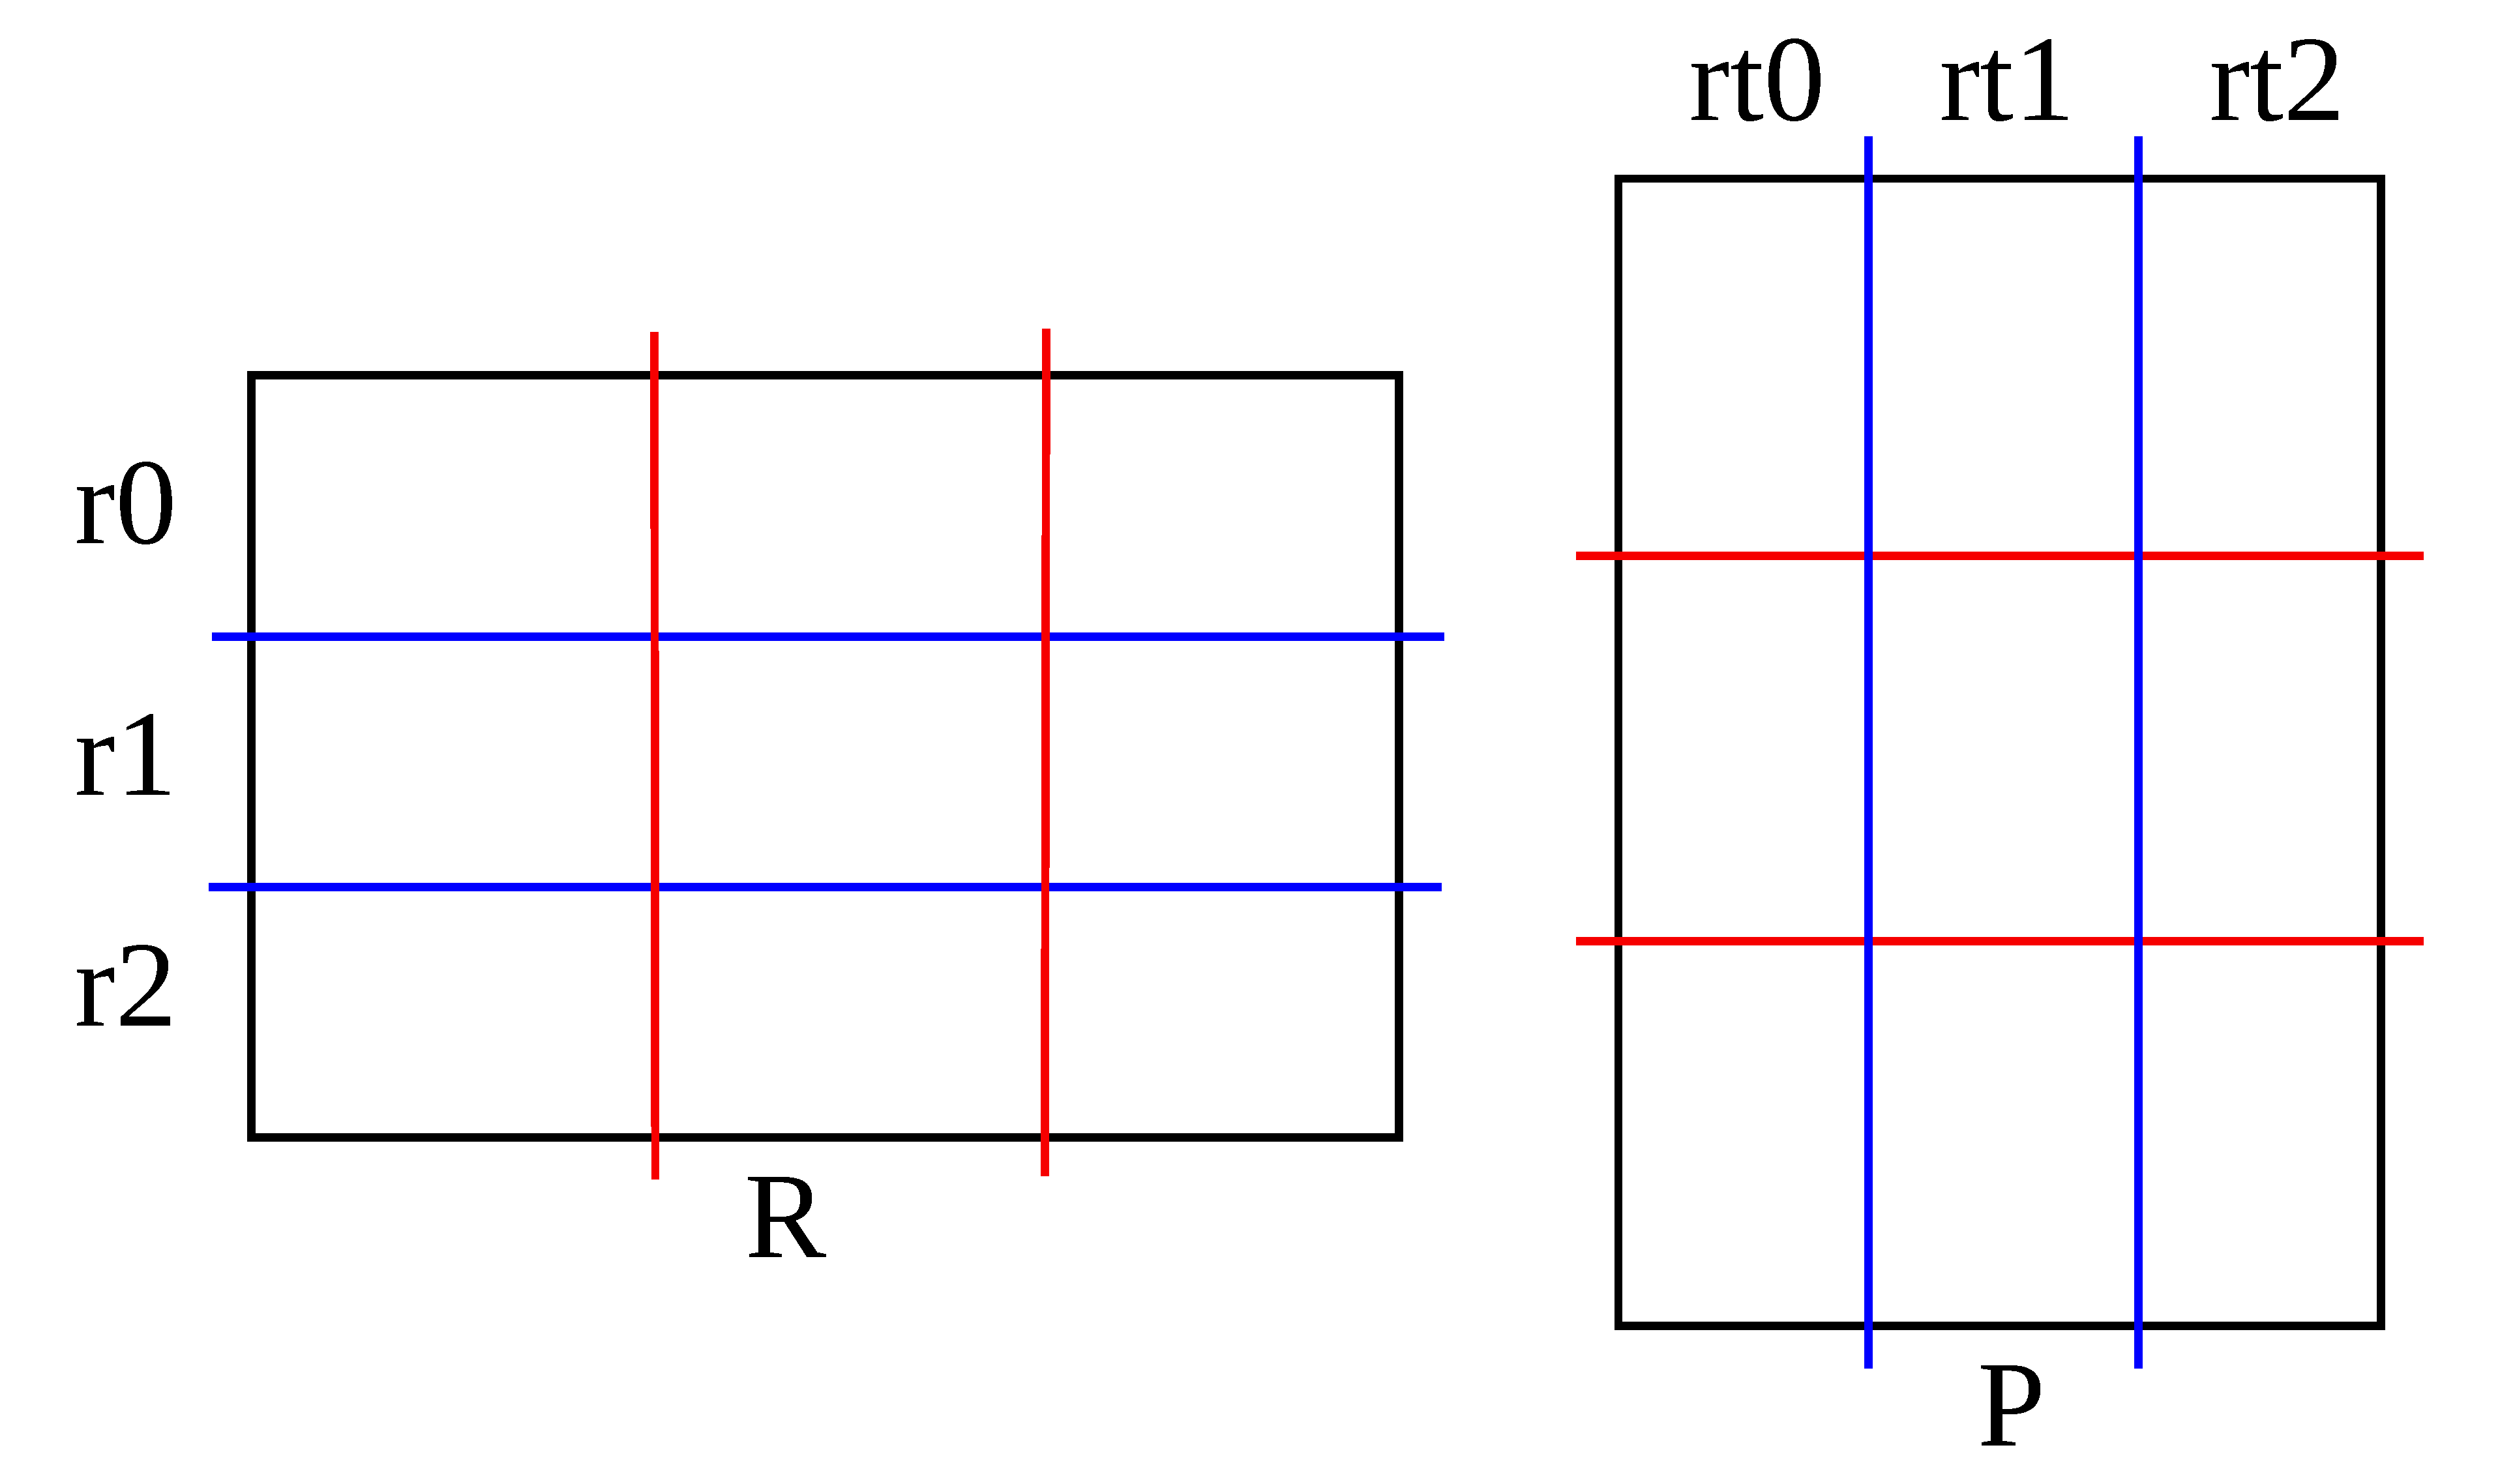
\includegraphics[width=5cm,height=2.9cm]{./figures/part1c.pdf}
    \caption{This figure shows how row blocks of $R$ are transpose of column blocks of $P$.}
    \label{fig:part1c}
    \Description{}
\end{figure}

Column $j$ of $P$ is distributed between all the processors. Therefore we need to communicate all nonzeros of that column and then perform $B_{ij} = \sum_{k} A_{ik} P_{kj}$. Since that can lead to significant communication, we make use of the fact that $R$ is the transpose of $P$ and is already available locally because of the multigrid hierarchy. We note that column blocks of $P$ (e.g. $r0$ in Figure~\ref{fig:part1c}) are actually row blocks of $R$ transposed ($rt0$, which is transpose of $r0$).

We have implemented this part in an overlapped fashion; first we do the send and receive commands (to communicate $rt$ blocks) and while this communication is being done, we perform \mm, so saving time for the communication (Algorithm \ref{alg:part1}). $B_{i}$ in the algorithm is the row block of matrix $B$ on processor $i$ and $B_{ik}$ is the sub-block result of multiplying $A_i$ with $rt_k$.

\iffalse
\begin{figure}[tbh]
 \centering
 %\Description{Description}
 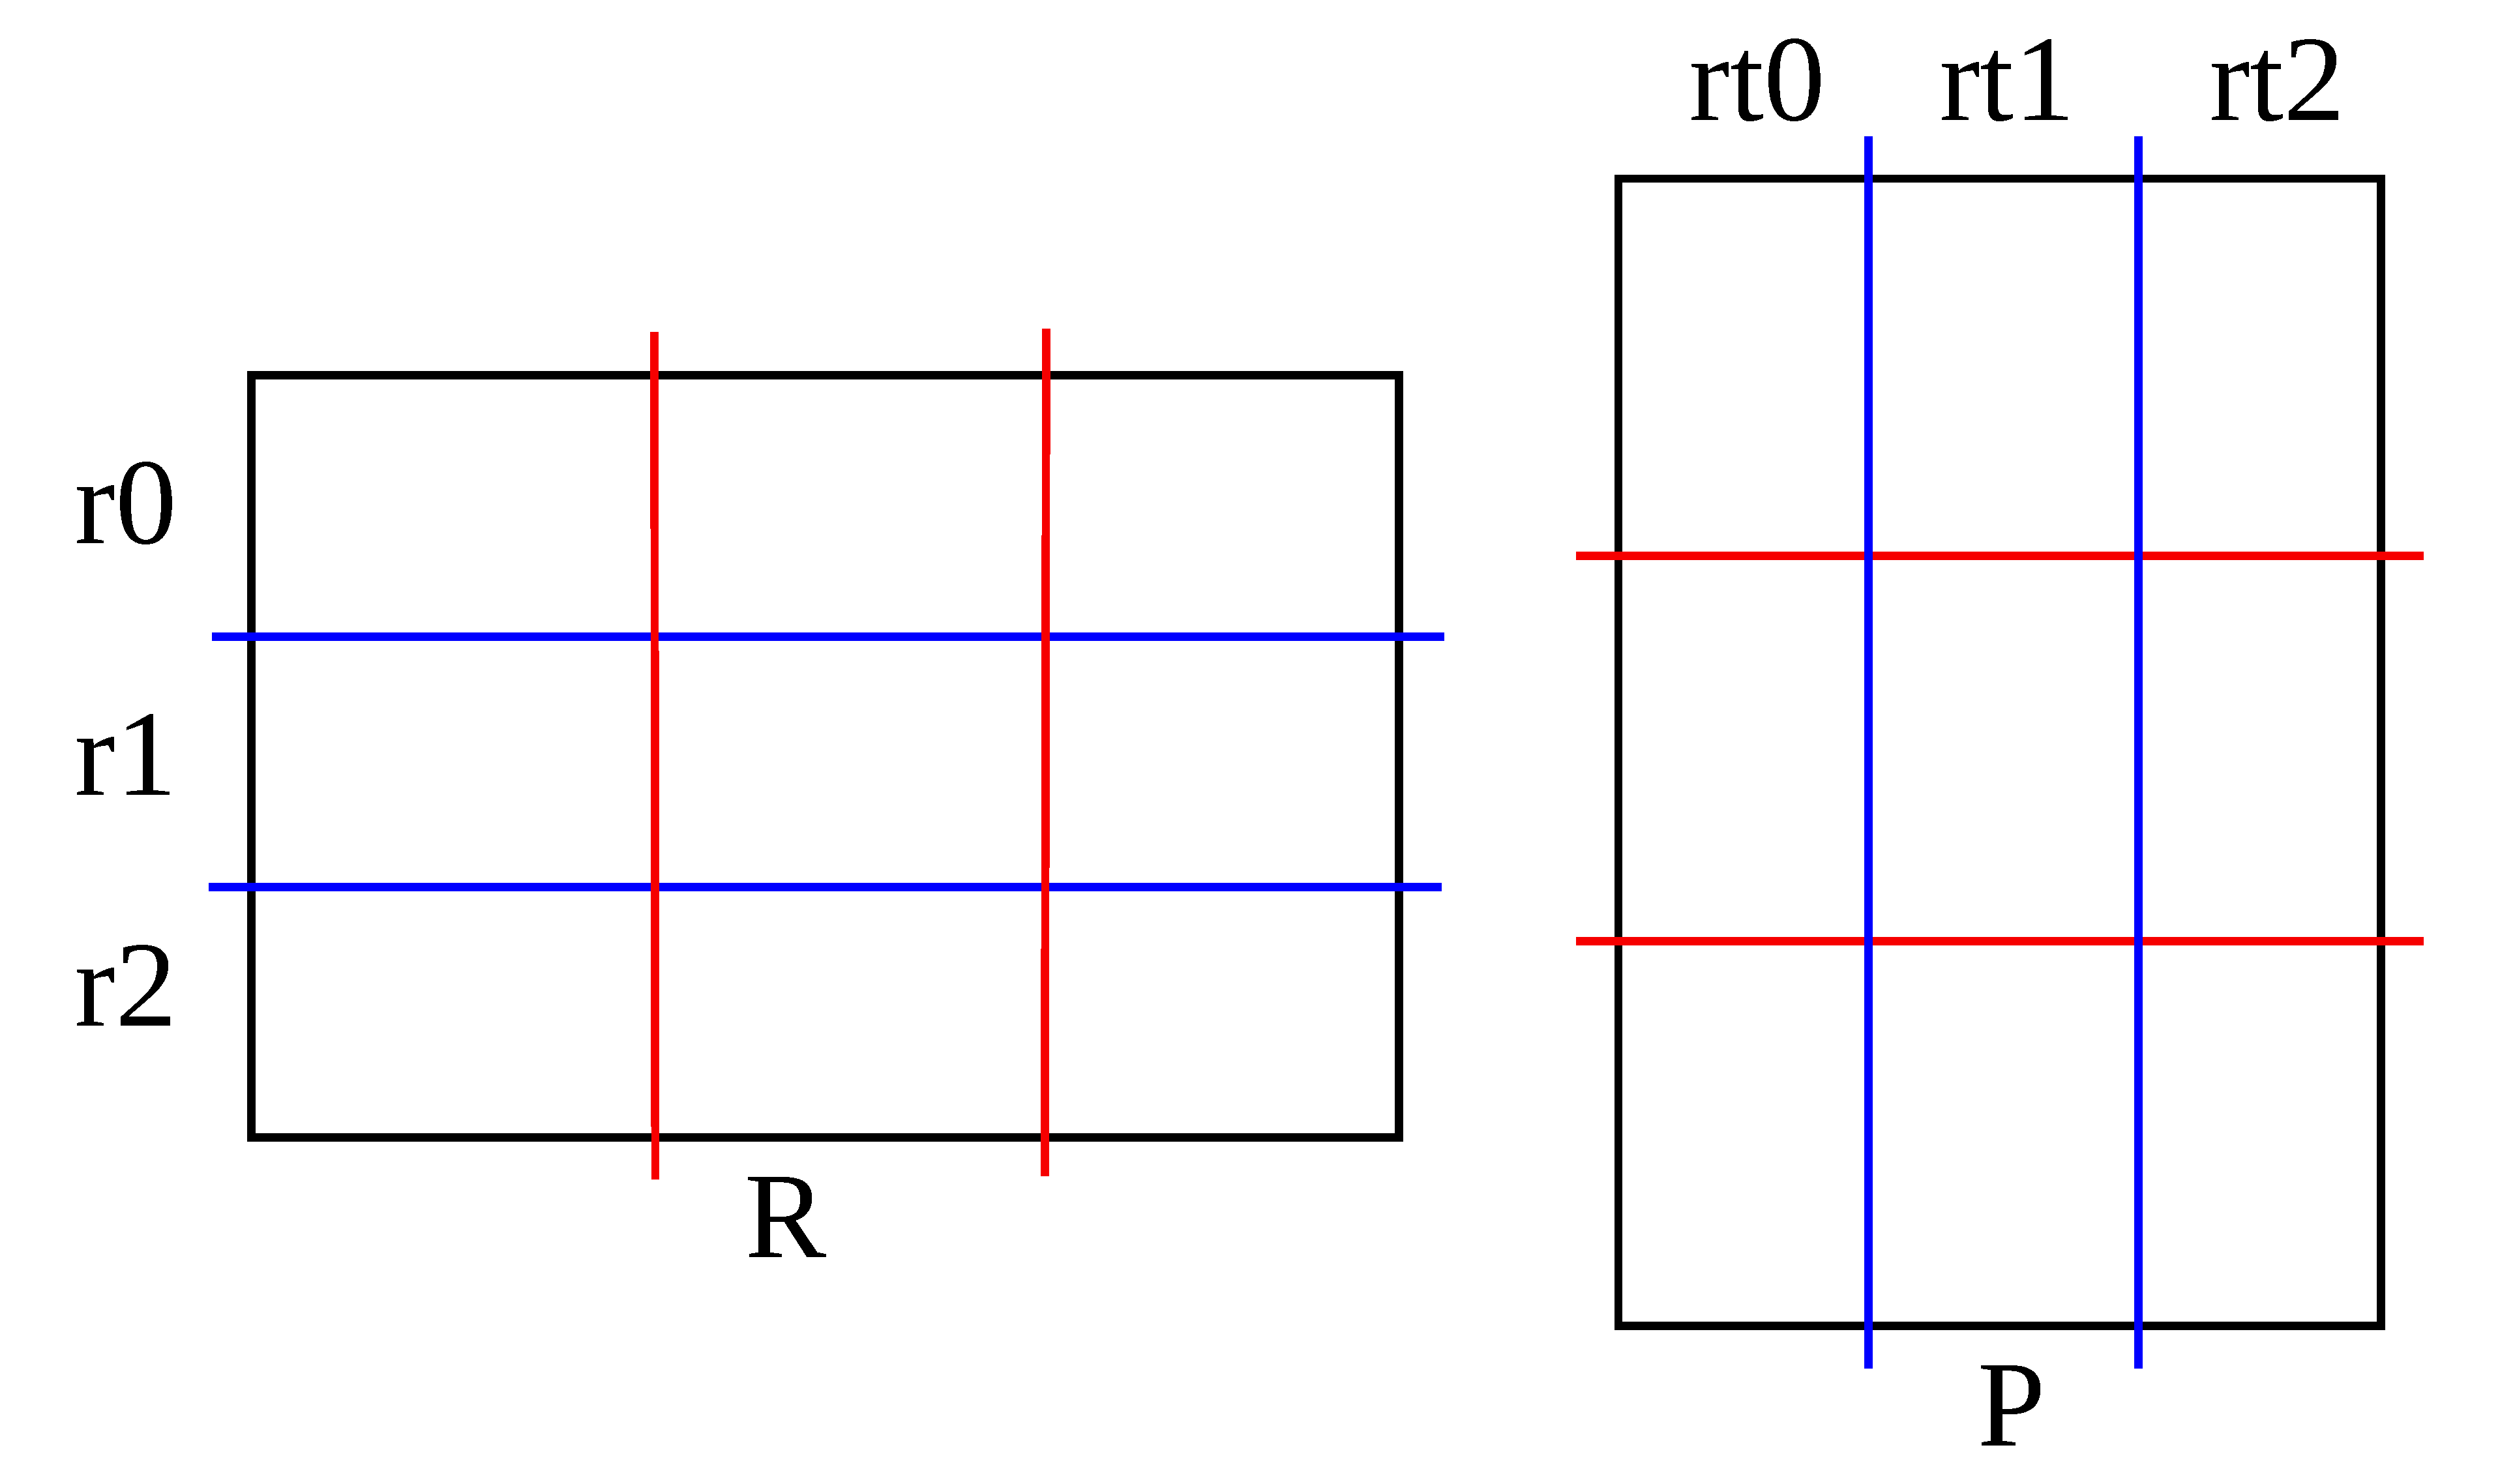
\includegraphics[width=5.5cm,height=3cm]{./figures/part1c.pdf}
 \caption{This figure shows how row blocks of $R$ are transpose of column blocks of $P$.}
 \label{fig:part1c}
\end{figure}
\fi

\begin{algorithm}[H] 
  %\footnotesize
  \caption{Part 1: $B_i = A_i \times P$} \label{alg:part1} 
  \begin{algorithmic}[1]
    \Require $A_i$, $R$
    \Ensure  $B_i$ (result of $A_i \times P$)
    \State $R1 \leftarrow$ transpose of $R_i$ (locally)
    \For{$k=myrank:myrank+nprocs$}
      \State $R2 \leftarrow\ Irecv(transpose\ of\ R block)\ from\ right\ neighbor$
      \State $Isend(R1)\ to\ left\ neighbor$
      \State $B_{ik} \leftarrow \recmm(A_i, R1)$ 
      \State $wait\ for\ Isend\ and\ Irecv\ to\ finish$
      \State $swap(R1,R2)$
    \EndFor
    \State locally sort $B_i$ and add duplicates
  \end{algorithmic}
\end{algorithm}

\section{Numerical Results}
\label{sec:results}

For our experiments we have used RMACC Summit Supercomputer in University of Colorado, Boulder. Each node has 24 cores and it uses Intel Xeon E5-2680 with $4.84GB$ of memory per core.

For these experiments for \mm~ we have multiplied a banded matrix with itself, assuming that the matrix is being multiplied with a separate matrix, so not using any information from the left-hand side matrix for the right-hand side one.

Figure\ref{fig:weak1} shows the weak scaling for two banded matrices.

\begin{figure}[tbh]
 \centering
 \Description{Description}
 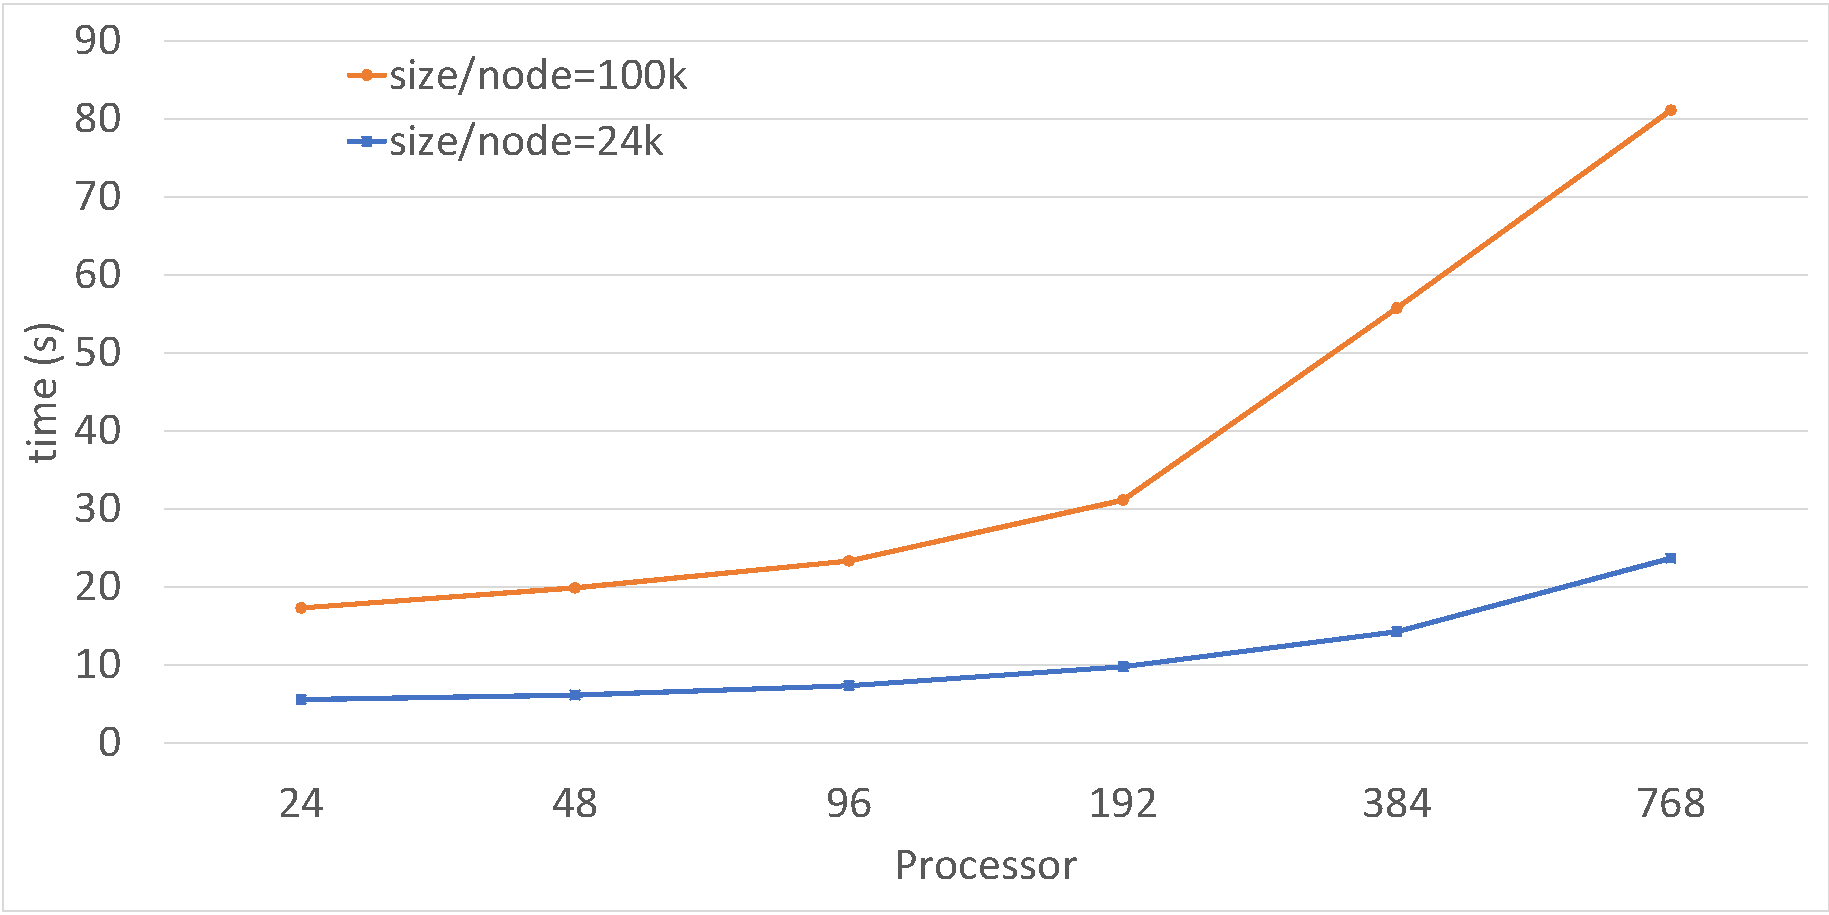
\includegraphics[width=8.5cm,height=4.8cm]{./figures/weak1.pdf}
 \caption{1}
 \label{fig:weak1}
\end{figure}

Figure\ref{fig:strong1} is the strong scaling for five banded matrices of the same size (192k), but with different bandwidth. The legend shows the density ($\frac{nonzero}{size^2}$) of each matrix.

\begin{figure}[tbh]
 \centering
 \Description{Description}
 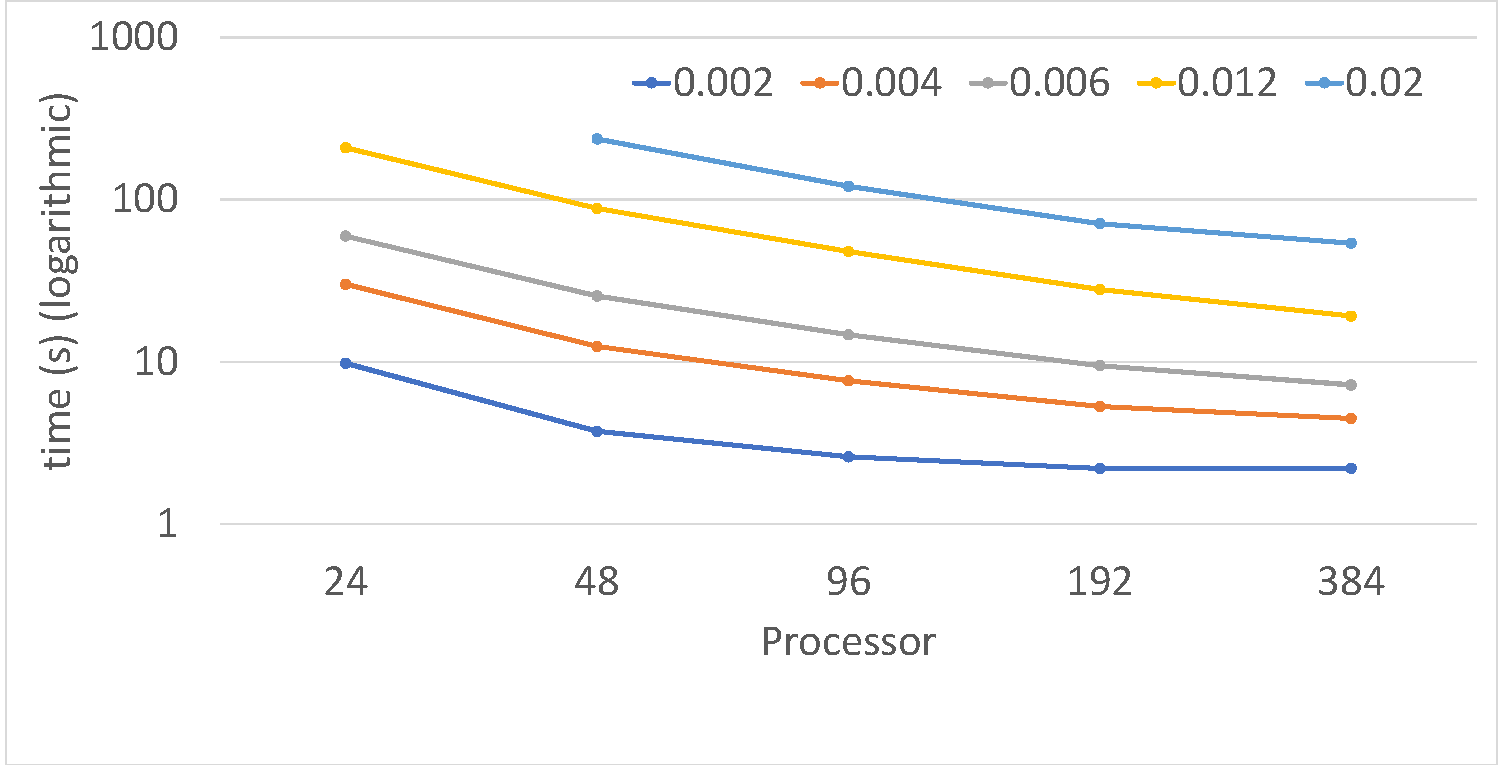
\includegraphics[width=8.5cm,height=4.9cm]{./figures/strong1.pdf}
 \caption{1}
 \label{fig:strong1}
\end{figure}

Figure\ref{fig:petsc1} compares the strong scaling between our solver and PETSc. For the matrices with lower density (more sparse) PETSc performs better when using higher number of processes, but for denser matrices our solver is faster. In multigrid hierarchy, the coarse matrices get denser as we go to lower levels, so it becomes expensive to perform \mm~ and having a fast matrix-matrix product would improve the setup cost significantly.

\begin{figure}[tbh]
 \centering
 \Description{Description}
 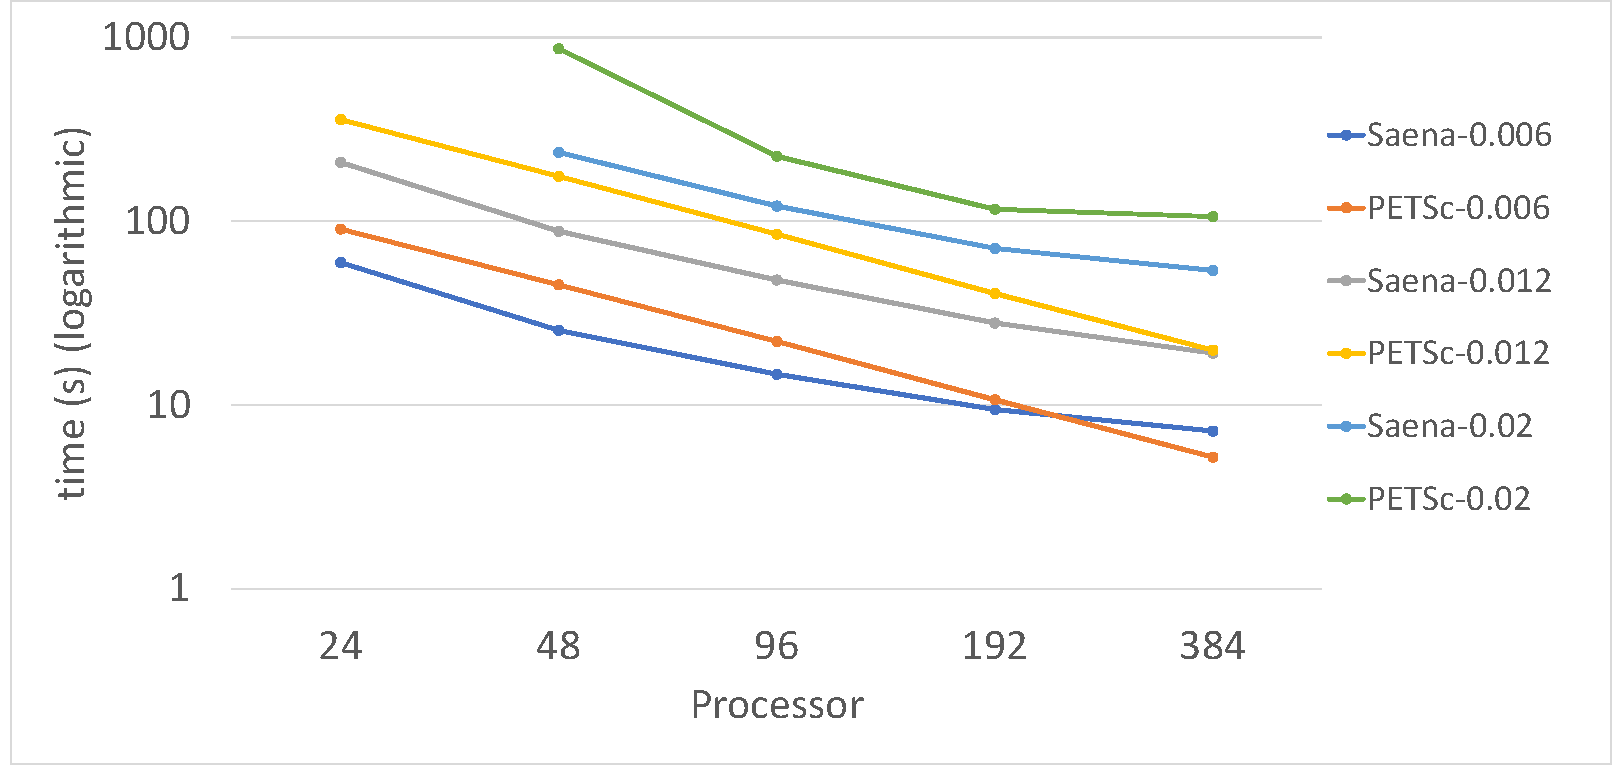
\includegraphics[width=8.5cm,height=4.4cm]{./figures/petsc1.pdf}
 \caption{1}
 \label{fig:petsc1}
\end{figure}



\bibliographystyle{splncs04}
\bibliography{references}

\end{document}



\iffalse
\section{First Section}
\subsection{A Subsection Sample}
Please note that the first paragraph of a section or subsection is
not indented. The first paragraph that follows a table, figure,
equation etc. does not need an indent, either.

Subsequent paragraphs, however, are indented.

\subsubsection{Sample Heading (Third Level)} Only two levels of
headings should be numbered. Lower level headings remain unnumbered;
they are formatted as run-in headings.

\paragraph{Sample Heading (Fourth Level)}
The contribution should contain no more than four levels of
headings. Table~\ref{tab1} gives a summary of all heading levels.

\begin{table}
\caption{Table captions should be placed above the
tables.}\label{tab1}
\begin{tabular}{|l|l|l|}
\hline
Heading level &  Example & Font size and style\\
\hline
Title (centered) &  {\Large\bfseries Lecture Notes} & 14 point, bold\\
1st-level heading &  {\large\bfseries 1 Introduction} & 12 point, bold\\
2nd-level heading & {\bfseries 2.1 Printing Area} & 10 point, bold\\
3rd-level heading & {\bfseries Run-in Heading in Bold.} Text follows & 10 point, bold\\
4th-level heading & {\itshape Lowest Level Heading.} Text follows & 10 point, italic\\
\hline
\end{tabular}
\end{table}


\noindent Displayed equations are centered and set on a separate
line.
\begin{equation}
x + y = z
\end{equation}
Please try to avoid rasterized images for line-art diagrams and
schemas. Whenever possible, use vector graphics instead (see
Fig.~\ref{fig1}).

\begin{figure}
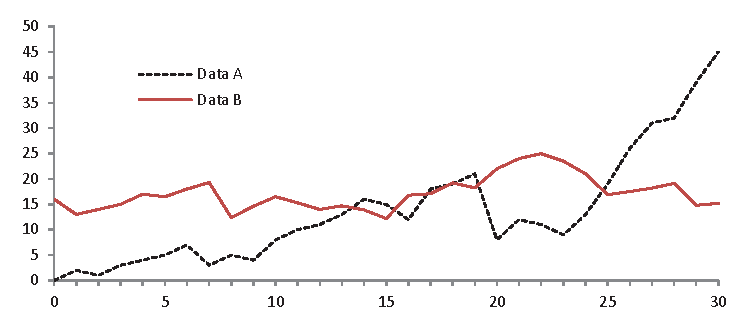
\includegraphics[width=\textwidth]{fig1.eps}
\caption{A figure caption is always placed below the illustration.
Please note that short captions are centered, while long ones are
justified by the macro package automatically.} \label{fig1}
\end{figure}

\begin{theorem}
This is a sample theorem. The run-in heading is set in bold, while
the following text appears in italics. Definitions, lemmas,
propositions, and corollaries are styled the same way.
\end{theorem}
%
% the environments 'definition', 'lemma', 'proposition', 'corollary',
% 'remark', and 'example' are defined in the LLNCS documentclass as well.
%
\begin{proof}
Proofs, examples, and remarks have the initial word in italics,
while the following text appears in normal font.
\end{proof}
For citations of references, we prefer the use of square brackets
and consecutive numbers. Citations using labels or the author/year
convention are also acceptable. The following bibliography provides
a sample reference list with entries for journal
articles~\cite{ref_article1}, an LNCS chapter~\cite{ref_lncs1}, a
book~\cite{ref_book1}, proceedings without editors~\cite{ref_proc1},
and a homepage~\cite{ref_url1}. Multiple citations are grouped
\cite{ref_article1,ref_lncs1,ref_book1},
\cite{ref_article1,ref_book1,ref_proc1,ref_url1}.
\fi


\iffalse
%
% ---- Bibliography ----
%
% BibTeX users should specify bibliography style 'splncs04'.
% References will then be sorted and formatted in the correct style.
%
% \bibliographystyle{splncs04}
% \bibliography{mybibliography}
%
\begin{thebibliography}{8}
\bibitem{ref_article1}
Author, F.: Article title. Journal \textbf{2}(5), 99--110 (2016)

\bibitem{ref_lncs1}
Author, F., Author, S.: Title of a proceedings paper. In: Editor,
F., Editor, S. (eds.) CONFERENCE 2016, LNCS, vol. 9999, pp. 1--13.
Springer, Heidelberg (2016). \doi{10.10007/1234567890}

\bibitem{ref_book1}
Author, F., Author, S., Author, T.: Book title. 2nd edn. Publisher,
Location (1999)

\bibitem{ref_proc1}
Author, A.-B.: Contribution title. In: 9th International Proceedings
on Proceedings, pp. 1--2. Publisher, Location (2010)

\bibitem{ref_url1}
LNCS Homepage, \url{http://www.springer.com/lncs}. Last accessed 4
Oct 2017
\end{thebibliography}


%\bibliographystyle{siamplain}
%\bibliography{references}

\end{document}
\fi
